\section{Tests on the prototypes and results}
\subsection{Preliminary tests at IRMA}
\begin{frame}
  \frametitle{Tests of silicon detector at IRMA}
  \begin{columns}
    \begin{column}{0.45\textwidth}
      IRMA (CSNSM/CNRS/Orsay):
      \begin{itemize}
        \item Ion implantation source
        \item $5$ to $190\,\mathrm{keV}$
        \item Many species
      \end{itemize}
      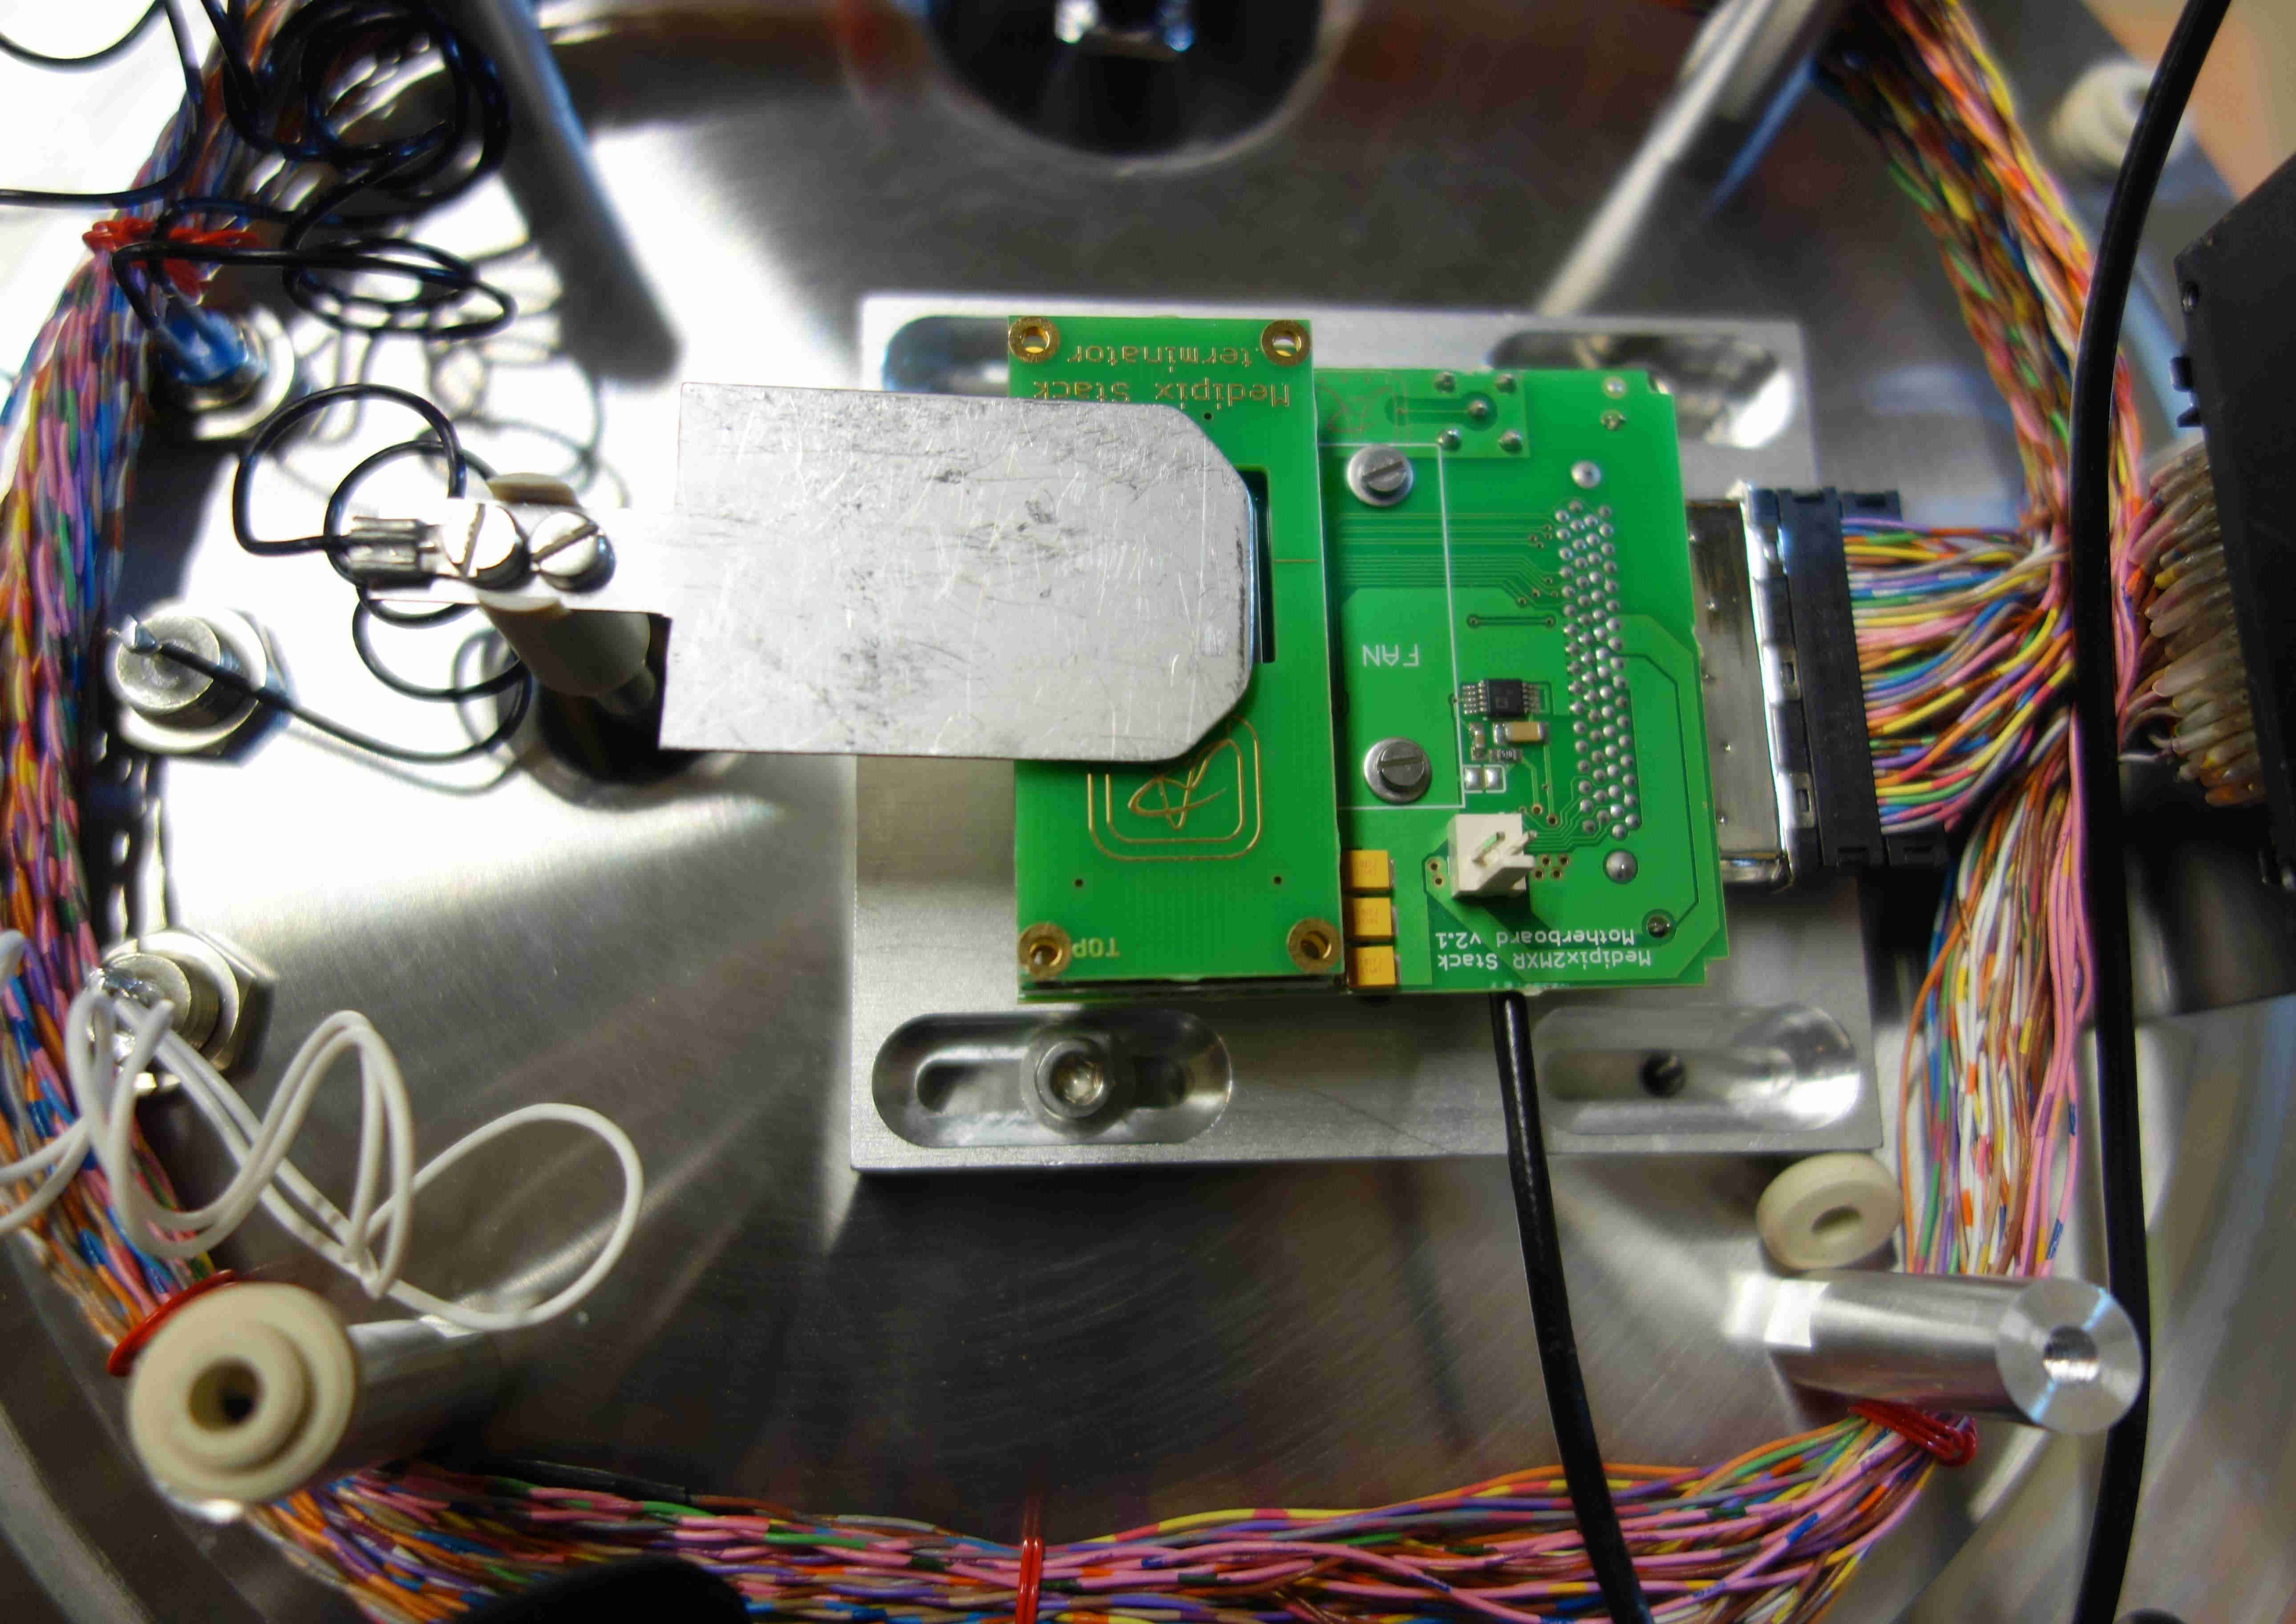
\includegraphics[width=\textwidth]{04_Test/fig/fig000_IRMA_setup01.jpg}
    \end{column}
    \begin{column}{0.45\textwidth}
      \begin{columns}
        \begin{column}{0.45\textwidth}
          \centering
          $15\,\mathrm{keV}$
          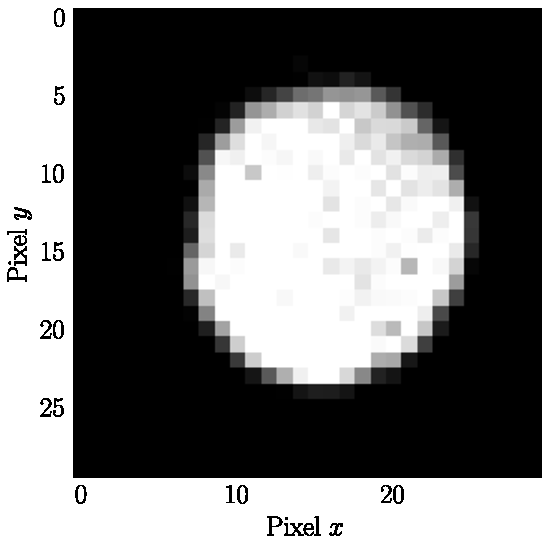
\includegraphics[width=0.8\textwidth]{04_Test/fig/fig000_IRMA_15keV_svg-tex.pdf}
        \end{column}
        \begin{column}{0.45\textwidth}
          \centering
          $12\,\mathrm{keV}$
          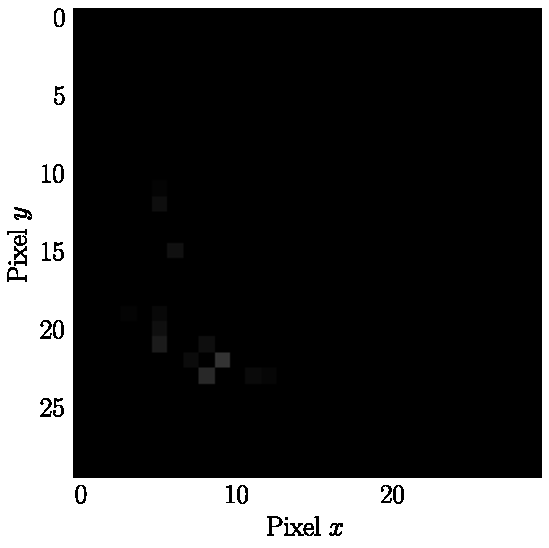
\includegraphics[width=0.8\textwidth]{04_Test/fig/fig000_IRMA_12keV_svg-tex.pdf}
        \end{column}
      \end{columns}
      \centering
      Damage after irradiation
      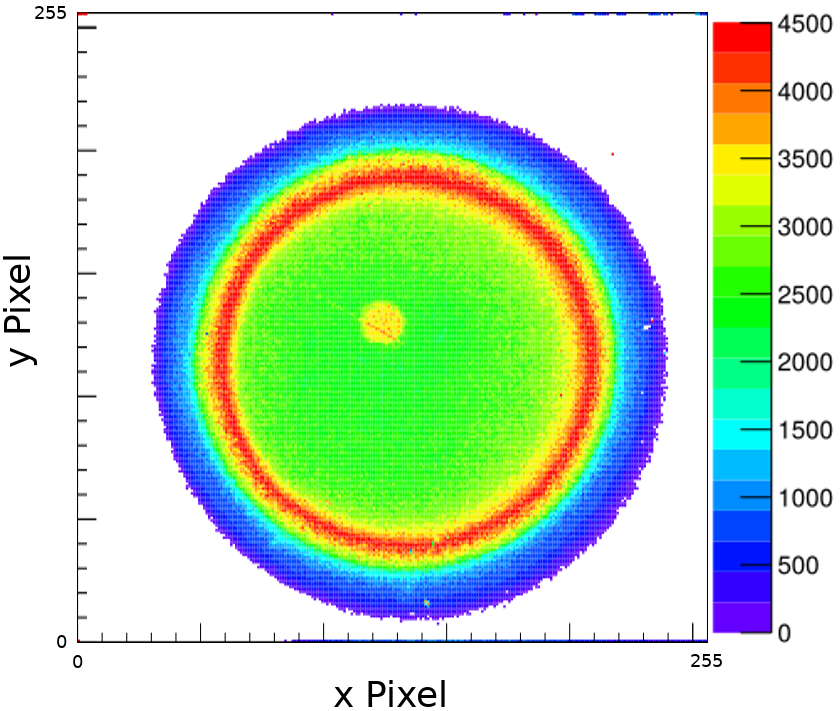
\includegraphics[width=0.8\textwidth]{04_Test/fig/fig000_IRMA_damage3.png}
    \end{column}
  \end{columns}
  \begin{alertblock}{It works but too risky}
    We discarded the silicon/TimePix option.
  \end{alertblock}
\end{frame}

\subsection{IPM testbench}
\begin{frame}
  \frametitle{IPM prototype}
  \begin{columns}
    \begin{column}{0.45\textwidth}
      \begin{block}{Prototype characteristics}
        \begin{itemize}
          \item Cage: $10\times10\times10\,\mathrm{cm}$
          \item Active area: $4\times2\,\mathrm{cm}$
          \item The readout can be easily changed.
        \end{itemize}
      \end{block}

      \begin{block}{Vacuum compliant materials}
        \begin{itemize}
          \item SS and copper
          \item Macor
          \item PEEK
          \item Ceramic PCB
        \end{itemize}
      \end{block}

    \end{column}
    \begin{column}{0.45\textwidth}
      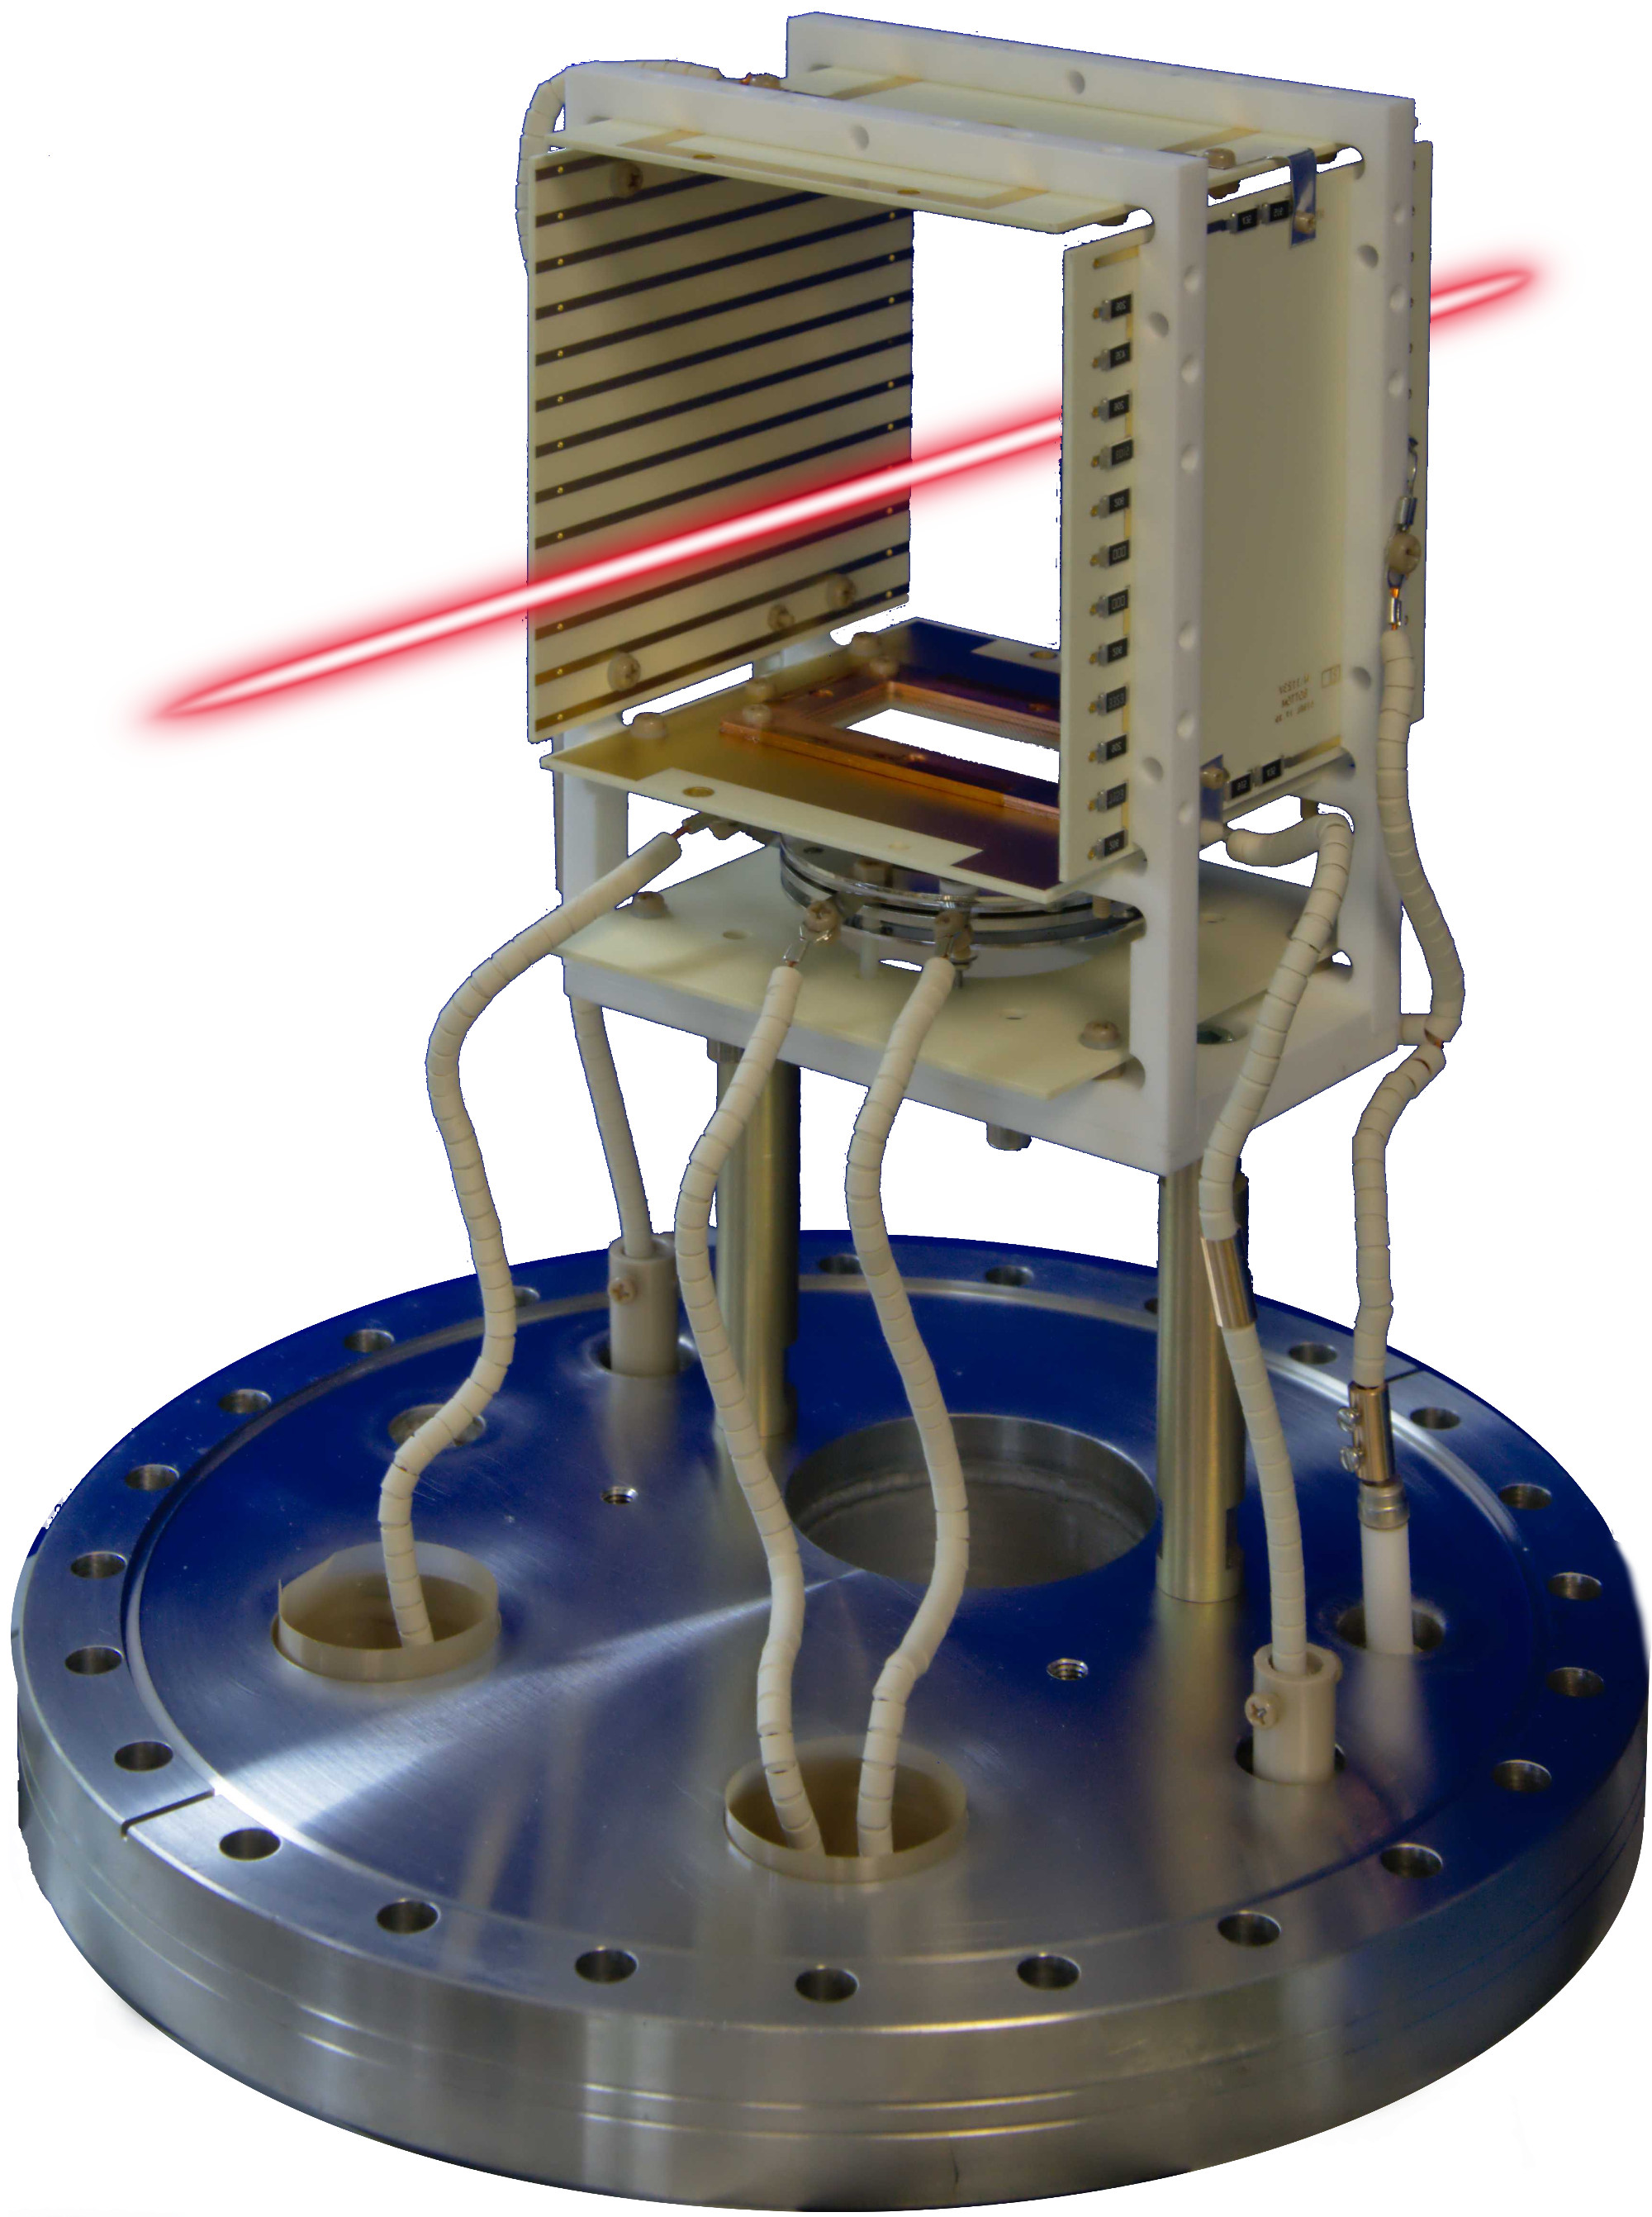
\includegraphics[width=\textwidth]{04_Test/fig/fig000_IPM_photo2}
    \end{column}
  \end{columns}
\end{frame}

\begin{frame}
  \frametitle{IPM test bench}
  As well, a dedicated test bench has been developed:
  \begin{center}
    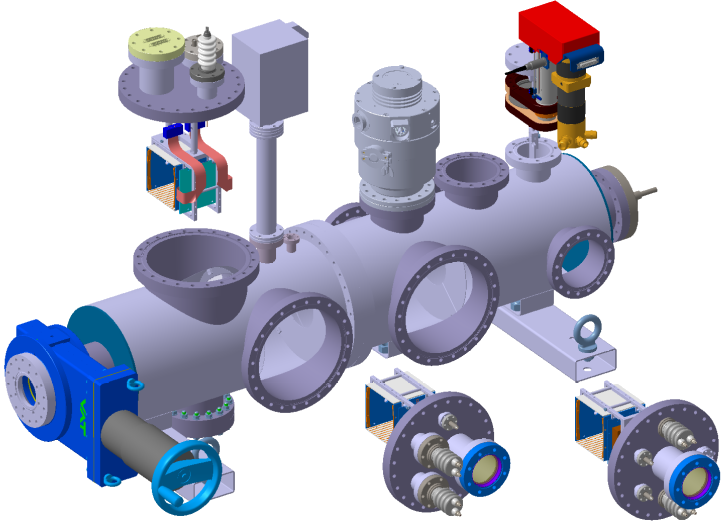
\includegraphics[width=0.7\textwidth]{04_Test/fig/fig000_Testbench2.png}
  \end{center}
  \begin{columns}[T]
    \begin{column}{0.45\textwidth}
      \begin{block}{Upstream}
        \begin{itemize}
          \item Mimic ESS LWU geometry.
          \item 2 slot for IPM prototypes.
        \end{itemize}
      \end{block}
    \end{column}

    \begin{column}{0.45\textwidth}
      \begin{block}{Downstream}
        \begin{itemize}
          \item Extension adding more slots.
          \item 1 slot for an IPM prototype.
          \item 2 slot for reference measurements.
        \end{itemize}
      \end{block}
    \end{column}
  \end{columns}

\end{frame}

\subsection{IPHI}
\begin{frame}
  \frametitle{IPHI}
  \begin{block}{Injecteur de Protons à Haute Intensité}
    IPHI is a high intensity $3\,\mathrm{MeV}$ proton accelerator at DACM/IRFU/CEA Saclay. IPHI can be seen as the 20 first meter of ESS.
  \end{block}
  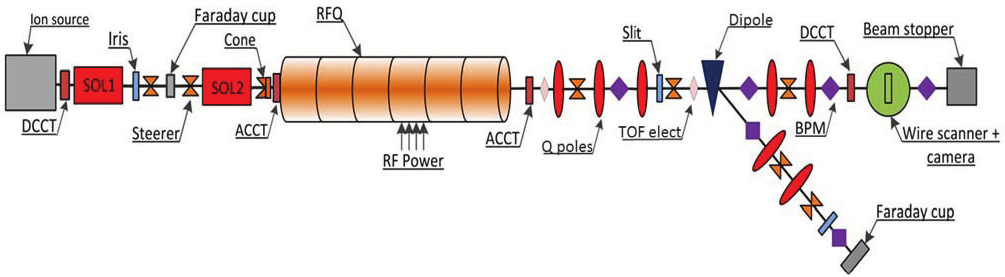
\includegraphics[width=1\textwidth]{04_Test/fig/fig000_IPHI_view.png}
  \begin{tabularx}{\linewidth}{XXX}
    \toprule
                         & IPHI accelerator                                  & ESS accelerator                \\
    \midrule
    Energy               & $3\,\mathrm{MeV}$                                 & $2\,\mathrm{GeV}$              \\
    Max current          & $0.5-100\,\mathrm{mA}$                            & $62.5\,\mathrm{mA}$            \\
    Max pulse duration   & $>100\,\mathrm{\mu s}$ up to DC                   & $2.86\,\mathrm{ms}$            \\
    Max pulse repetition & -                                                 & $14\,\mathrm{Hz}$              \\
    Vacuum range         & $5\cdot10^{-7}$ to $1\cdot10^{-8}\,\mathrm{mbar}$ & $1\cdot10^{-9}\,\mathrm{mbar}$ \\
    \bottomrule
  \end{tabularx}
\end{frame}

\begin{frame}[t]
  \frametitle{IPHI test campaign}
  \begin{block}{Goals:}
    \begin{itemize}
      \item Find out the most
      \item Characterize our prototypes
      \item Find flaws in your design
    \end{itemize}
  \end{block}
  \begin{columns}[T]
    \begin{column}{0.45\textwidth}
      \centering
      IPHI installation
      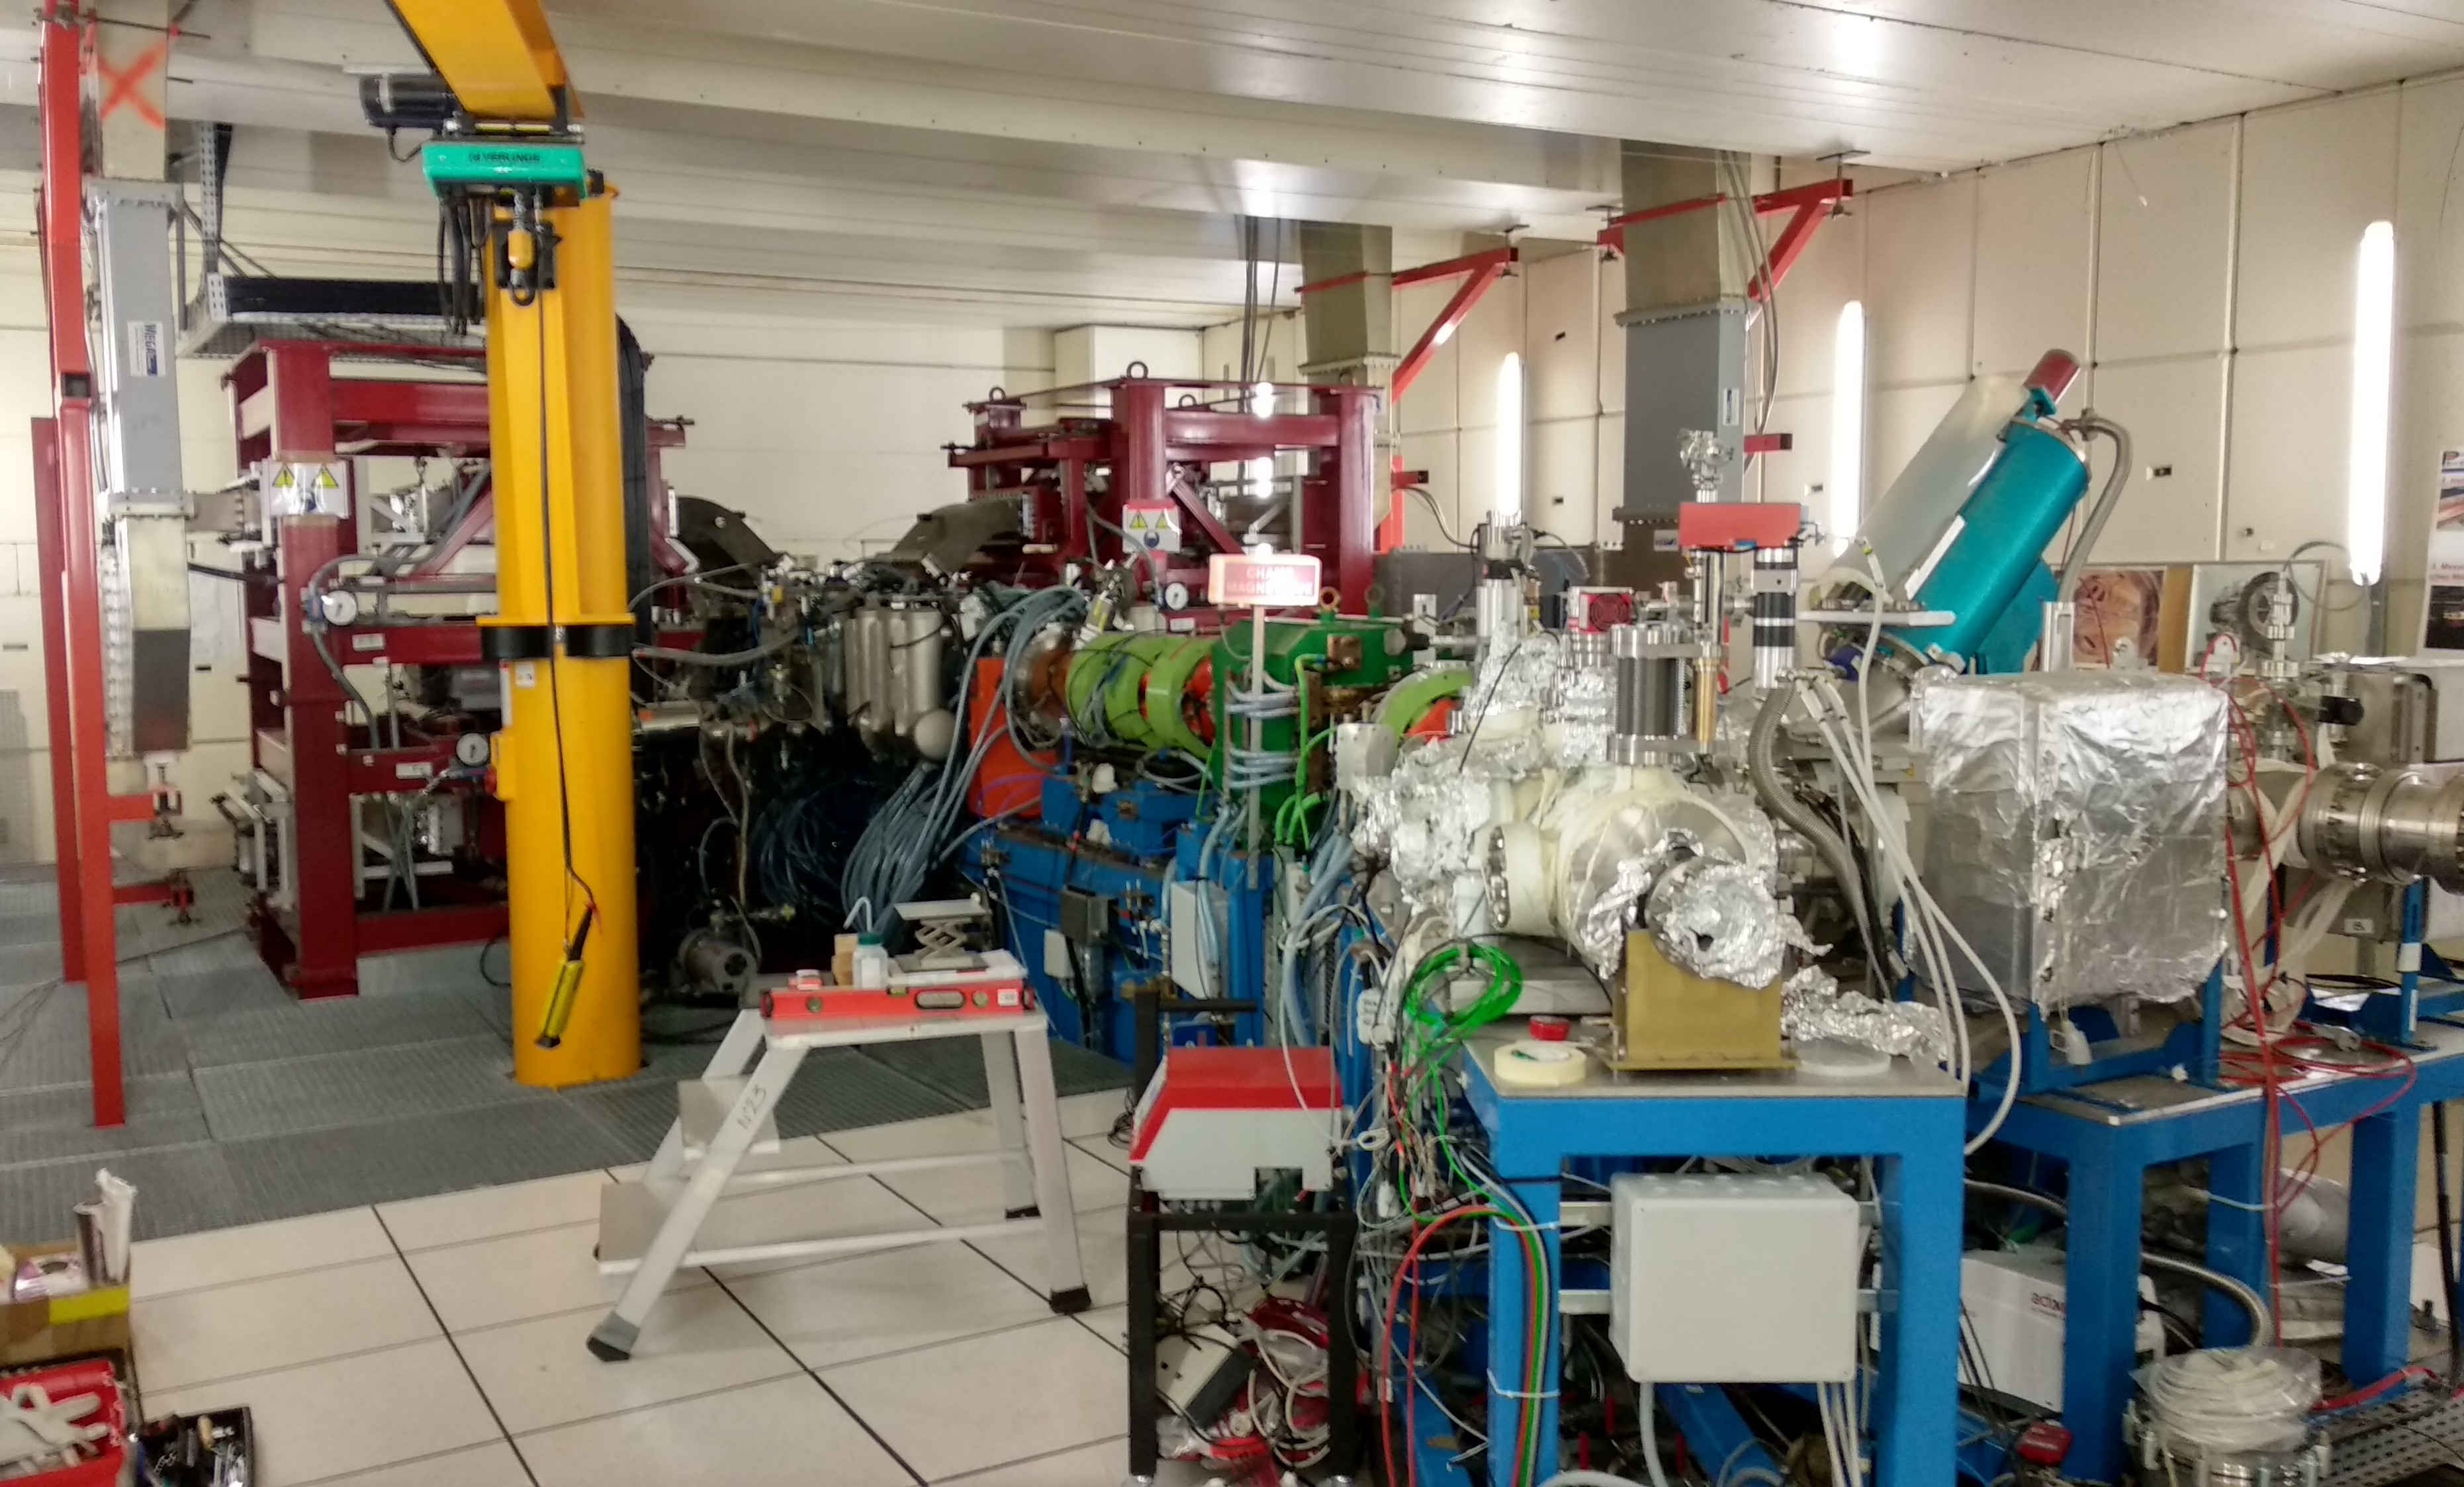
\includegraphics[width=1\textwidth]{04_Test/fig/fig000_IPHI_tb1.jpg}
    \end{column}
    \begin{column}{0.45\textwidth}
      \centering
      IPM test bench at IPHI
      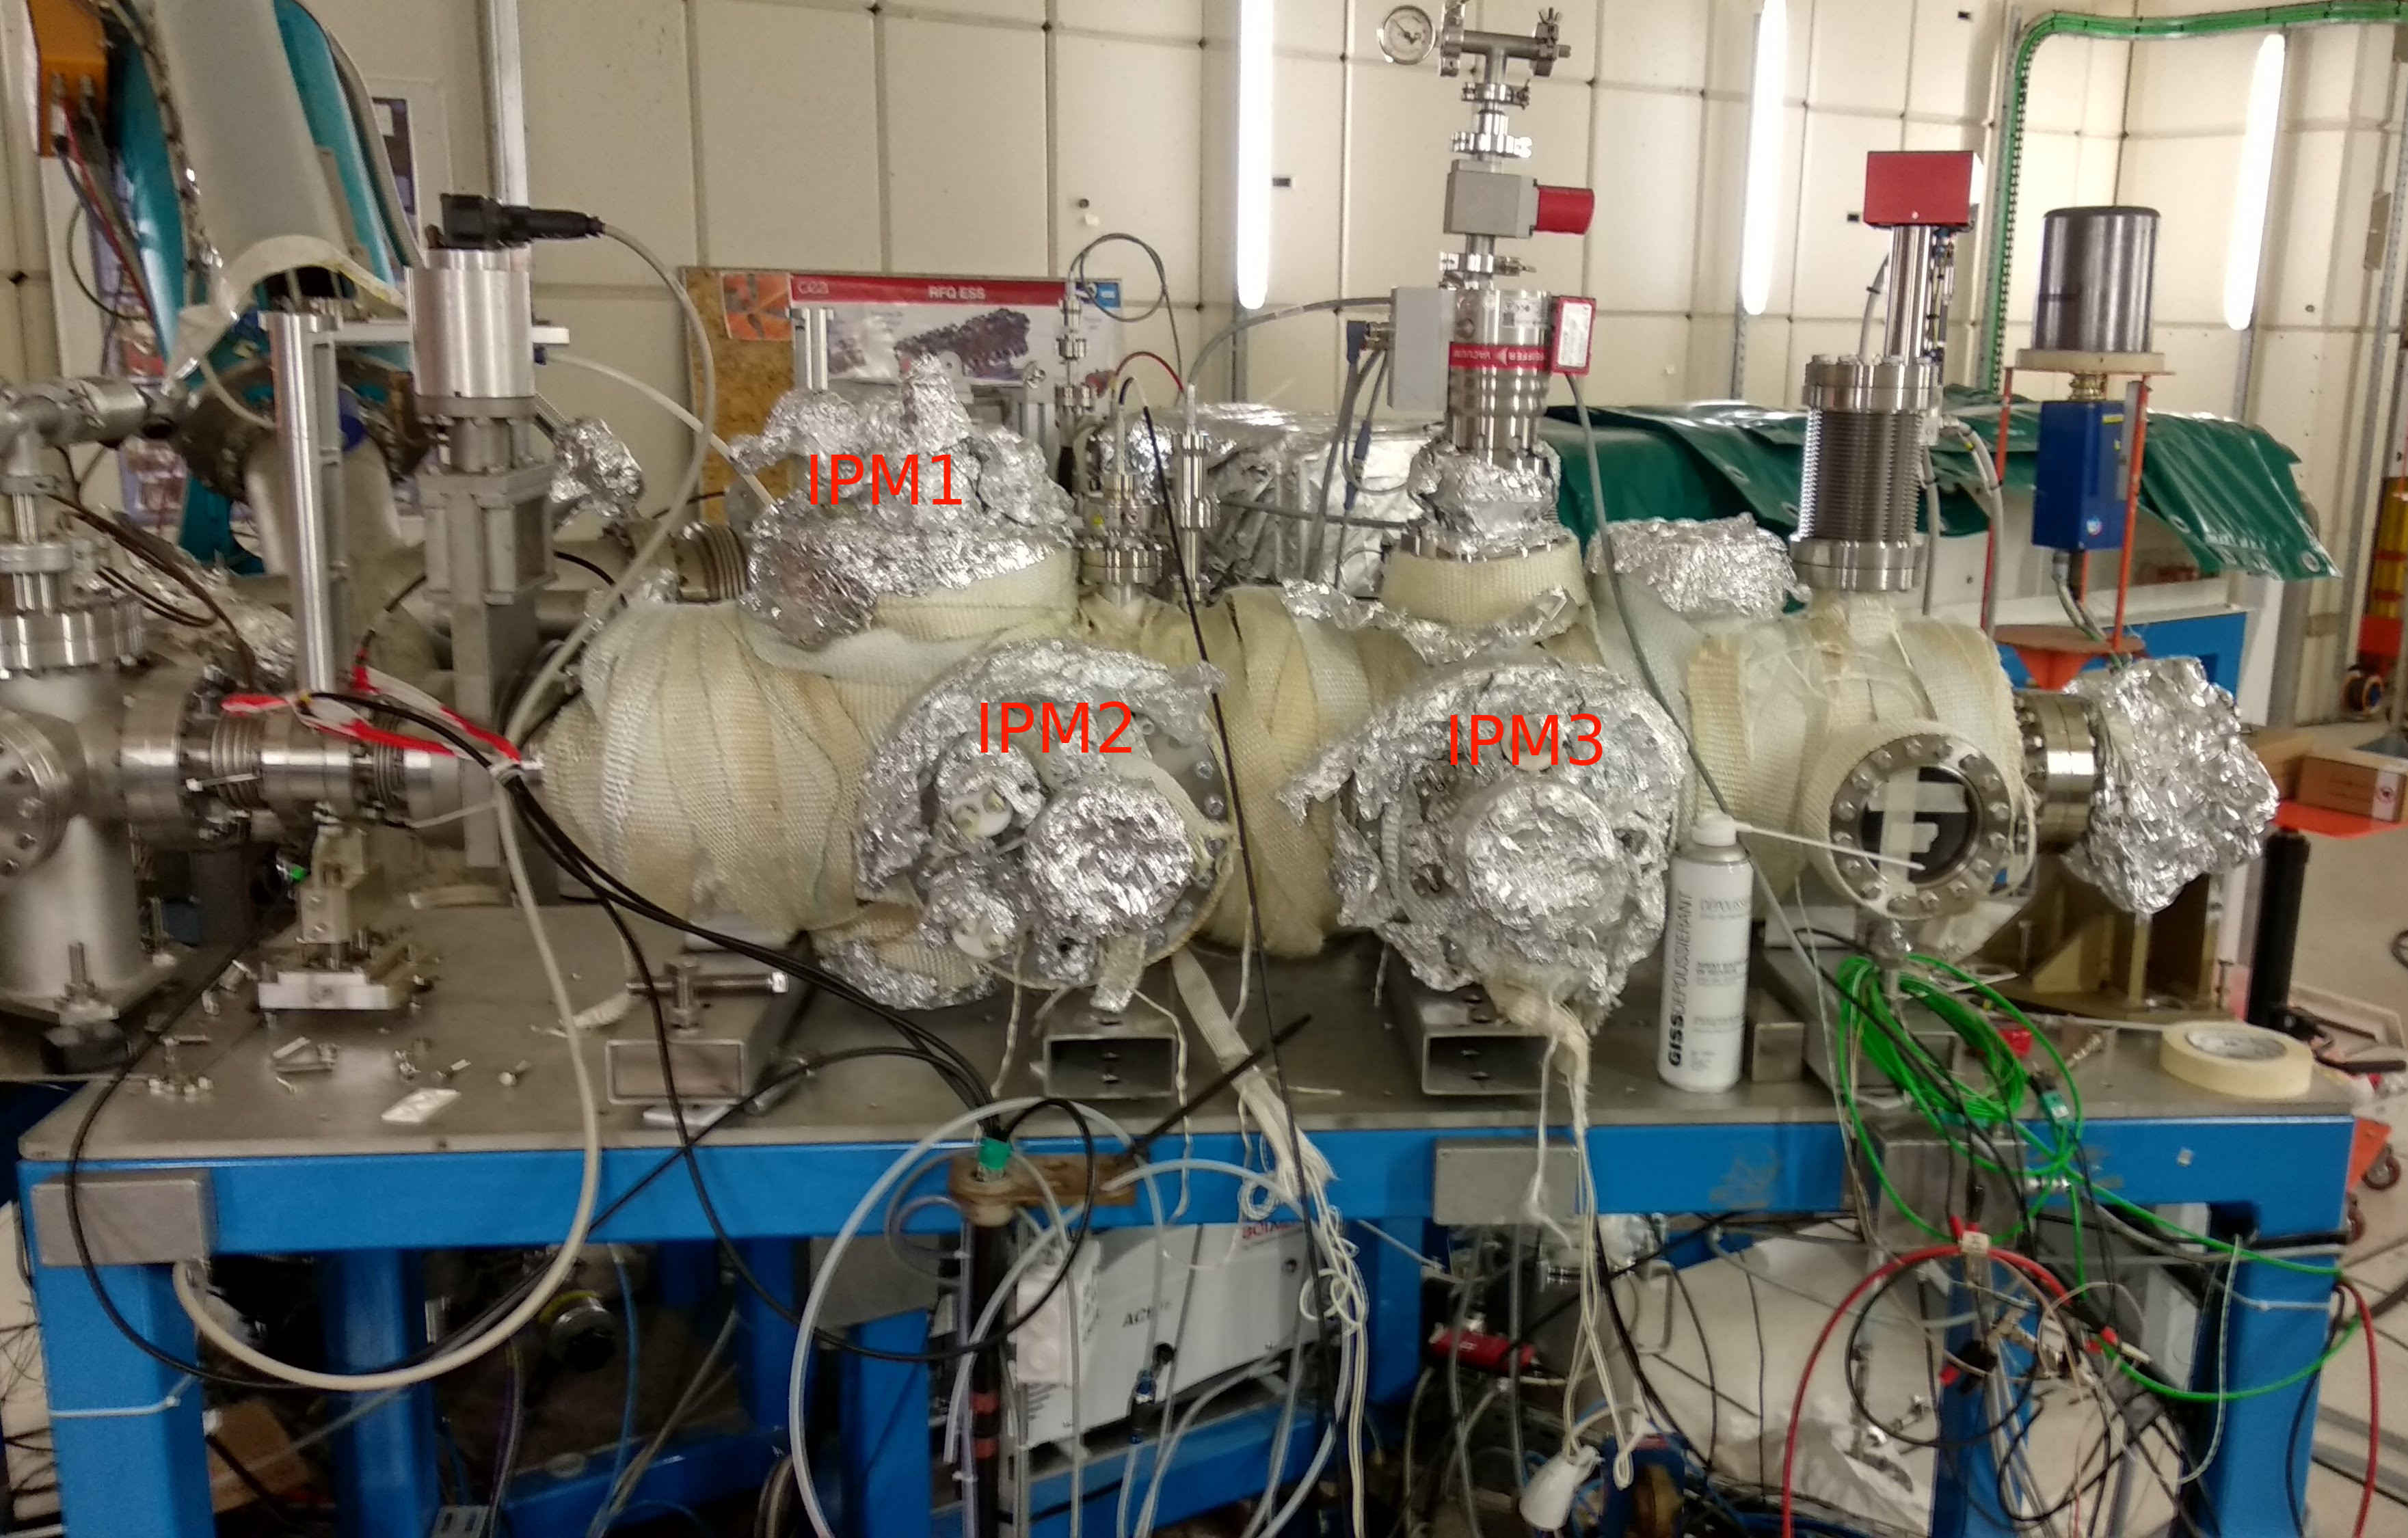
\includegraphics[width=1\textwidth]{04_Test/fig/fig000_IPHI_tb2.jpg}
    \end{column}
  \end{columns}
  \begin{block}{Two campaigns:}
    \begin{itemize}
      \item First campaign: first tests but limited by spark issues
      \item Second campaign:  improved prototypes, check limits.
    \end{itemize}
  \end{block}

  % \begin{tabularx}{\linewidth}{XXX}
  %   \toprule
  %                 & First campaign & Second campaign \\
  %   \midrule
  %   Starting date & 19/02/2018     & 14/09/2018      \\
  %   First profile & 01/03/2018     & 14/09/2018      \\
  %   Ending date   & 13/04/2018     & 26/10/2018      \\
  %   \bottomrule
  % \end{tabularx}
\end{frame}

\subsection{Results}
\begin{frame}
  \frametitle{Processing data}
  \begin{columns}[T]
    \begin{column}{0.45\textwidth}
      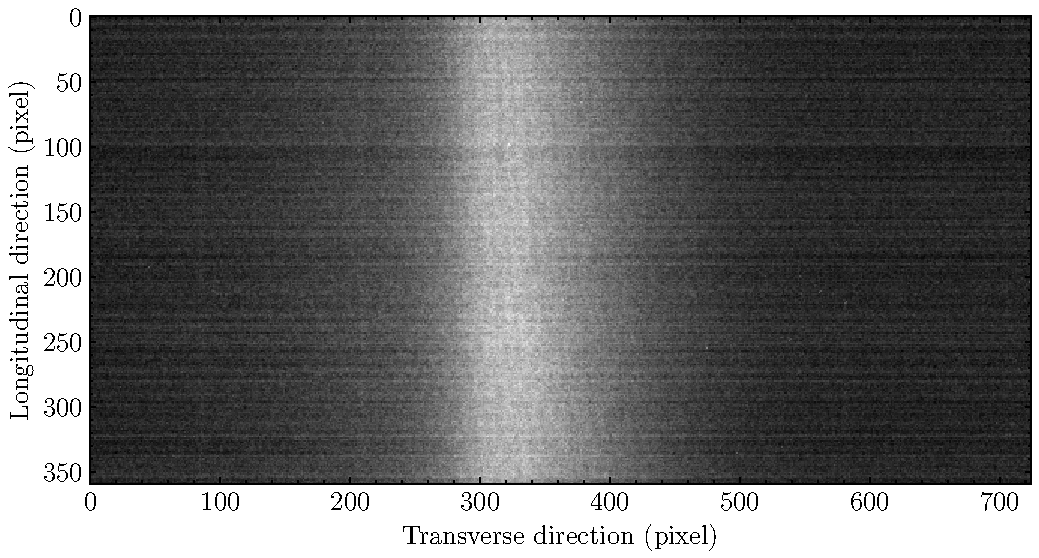
\includegraphics[width=1\textwidth]{04_Test/fig/fig000_image_beam}
    \end{column}
    \begin{column}{0.45\textwidth}
      \only<1>{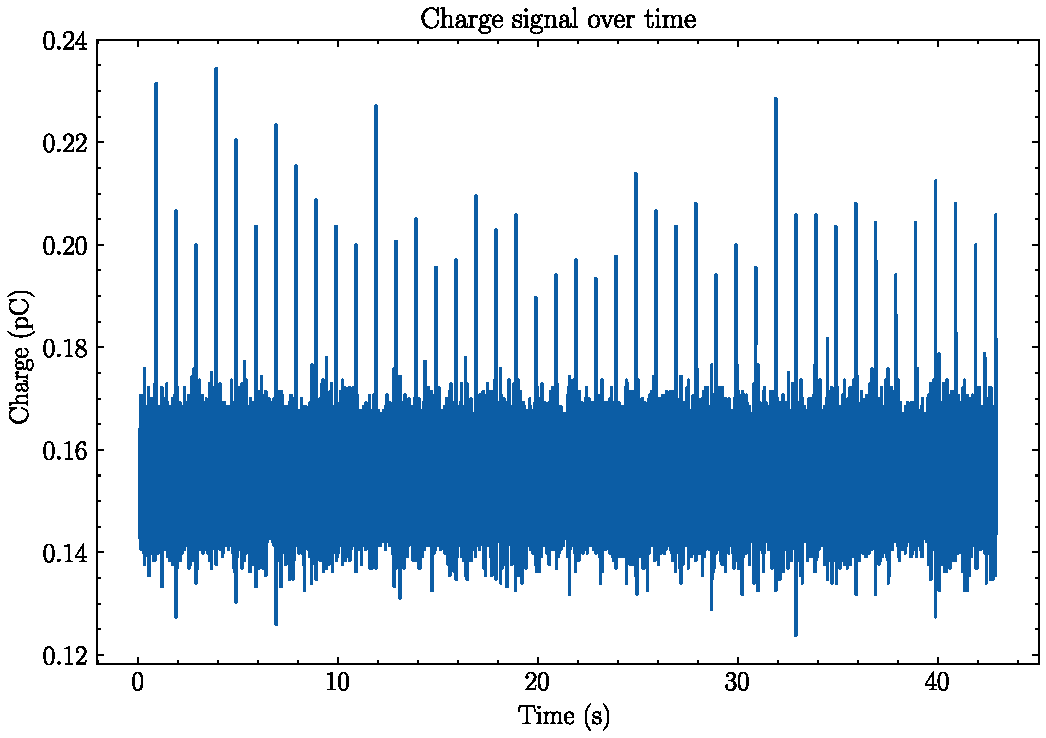
\includegraphics[width=1\textwidth]{04_Test/fig/fig000_strips_signal}}
      \only<2>{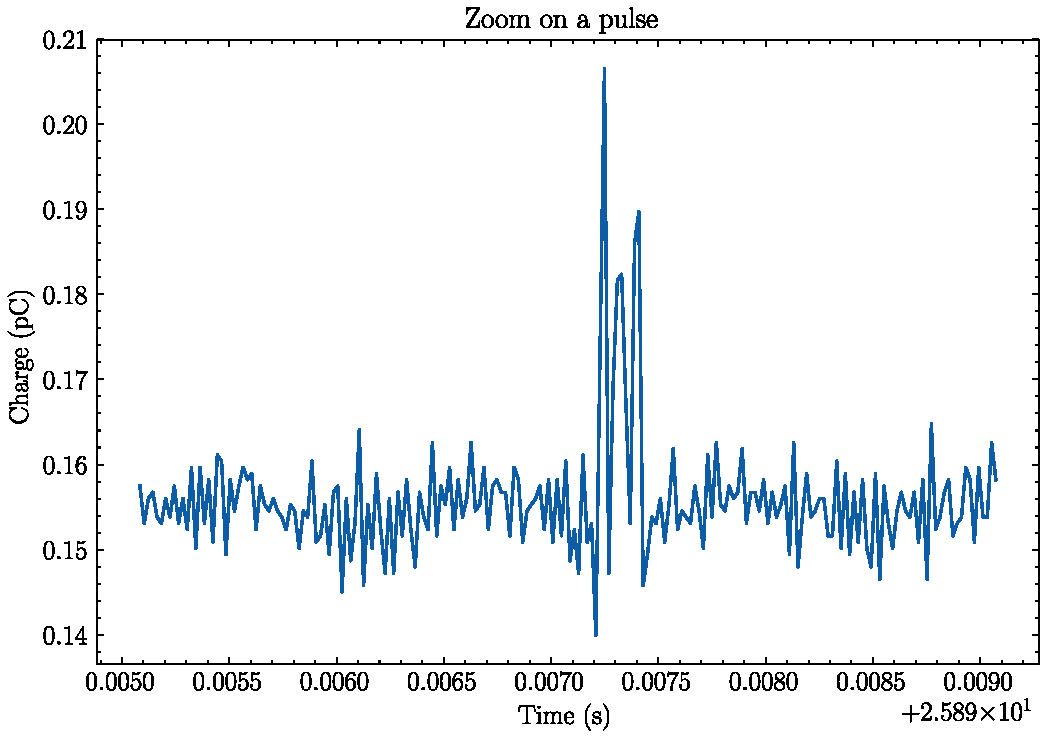
\includegraphics[width=1\textwidth]{04_Test/fig/fig000_strips_signal_b}}
    \end{column}
  \end{columns}
  \begin{columns}[T]
    \begin{column}{0.45\textwidth}
      \begin{block}{Processing}
        \begin{enumerate}
          \item Crop image to ROI
          \item Remove dead pixel
          \item Filtering
          \item Sum along longitudinal direction
        \end{enumerate}
      \end{block}
    \end{column}
    \begin{column}{0.45\textwidth}
      \begin{block}{Processing}
        \begin{enumerate}
          \item Remove pedestal
          \item Filtering
          \item Event finding with threshold
          \item Check multiplicity on several strips
        \end{enumerate}
      \end{block}
    \end{column}
  \end{columns}
\end{frame}

\begin{frame}
  \frametitle{Profile comparison between IPM}

  \begin{center}
    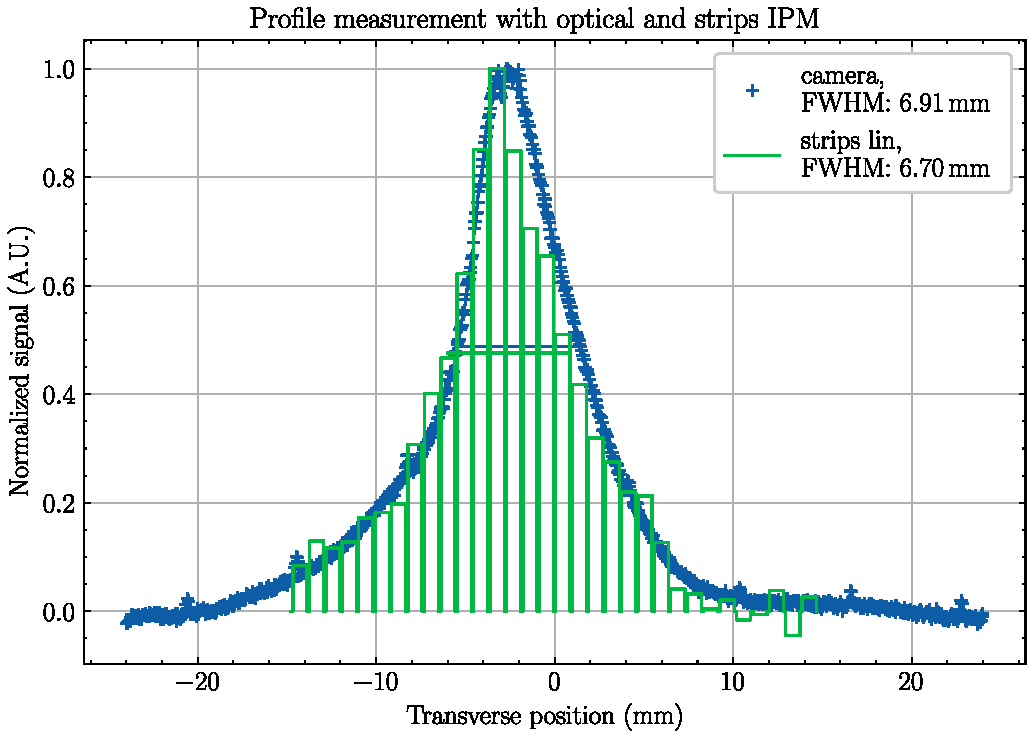
\includegraphics[width=0.75\textwidth]{04_Test/fig/fig000_MCP_strip}
  \end{center}
\end{frame}

\begin{frame}
  \frametitle{Limitations}
  \begin{columns}[T]
    \begin{column}{0.45\textwidth}
      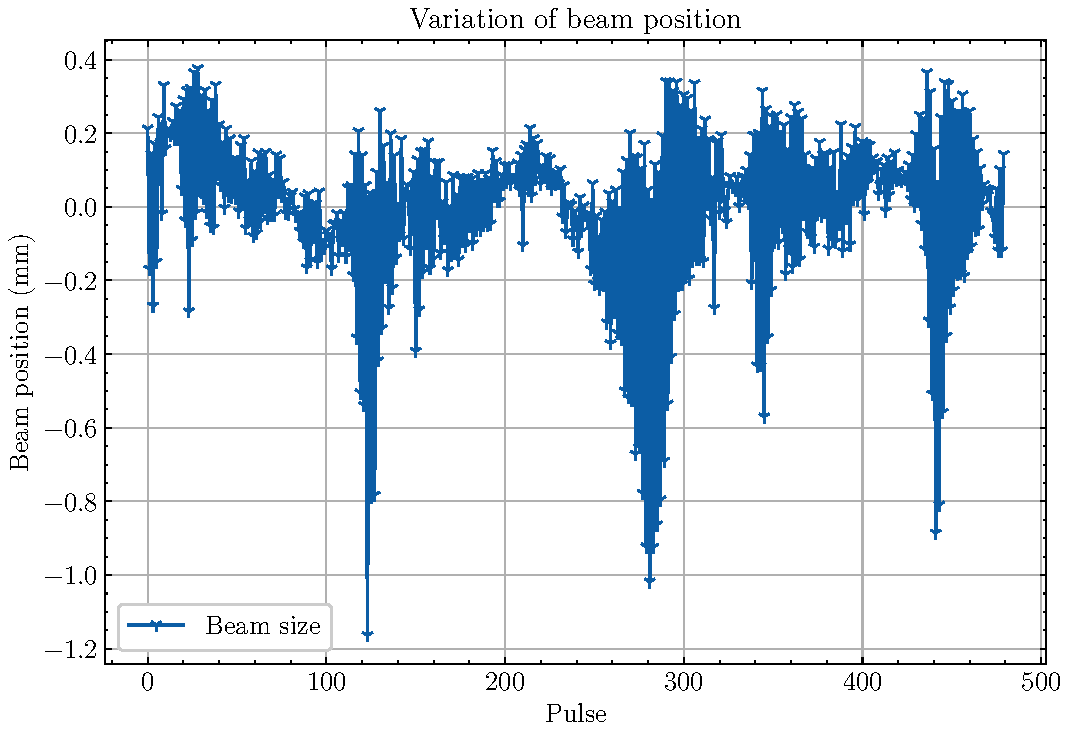
\includegraphics[width=1\textwidth]{04_Test/fig/fig000_variation_a}
      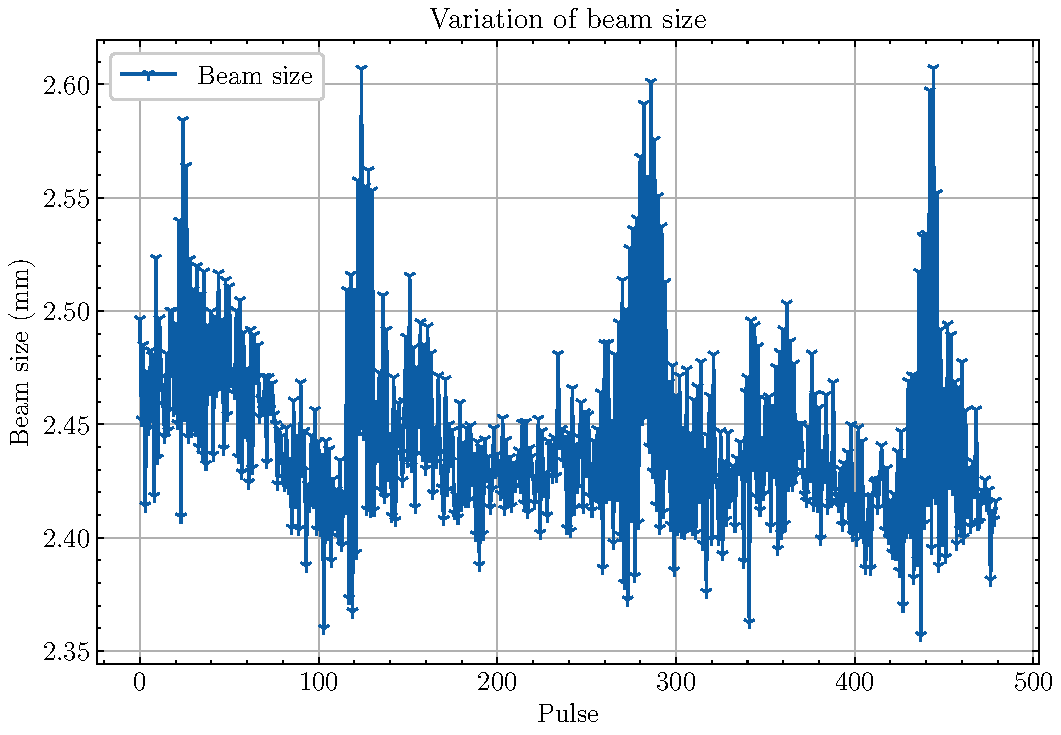
\includegraphics[width=1\textwidth]{04_Test/fig/fig000_variation_b}
    \end{column}
    \begin{column}{0.45\textwidth}
      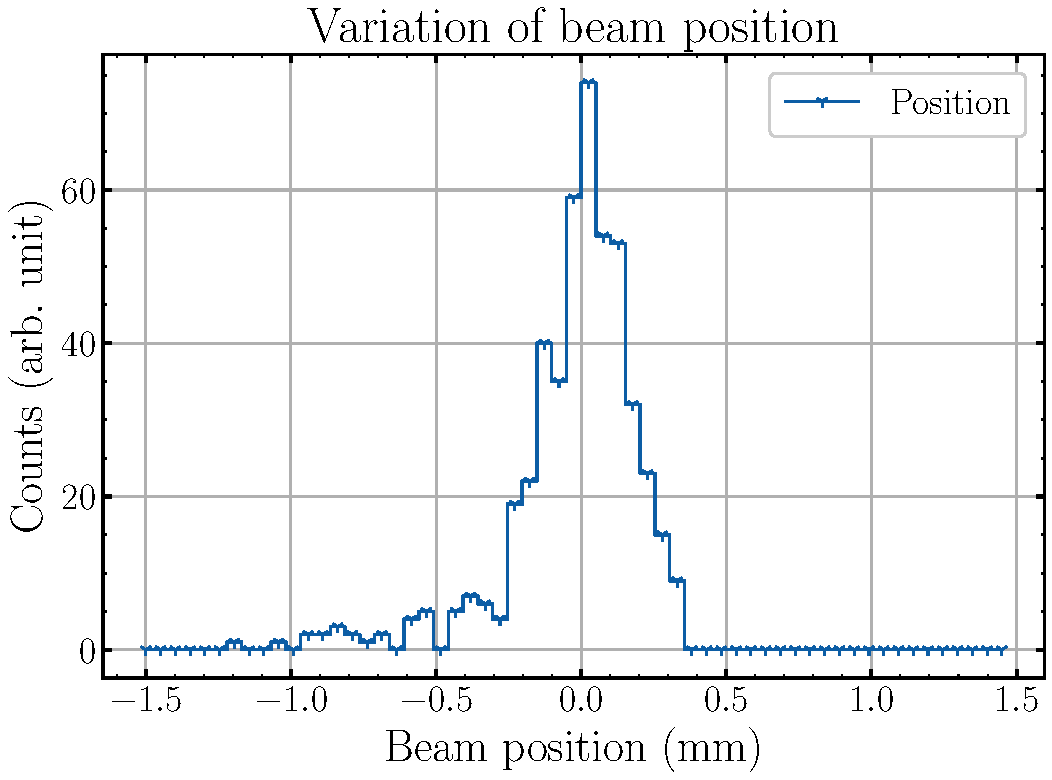
\includegraphics[width=1\textwidth]{04_Test/fig/fig000_hist_variation_a}
      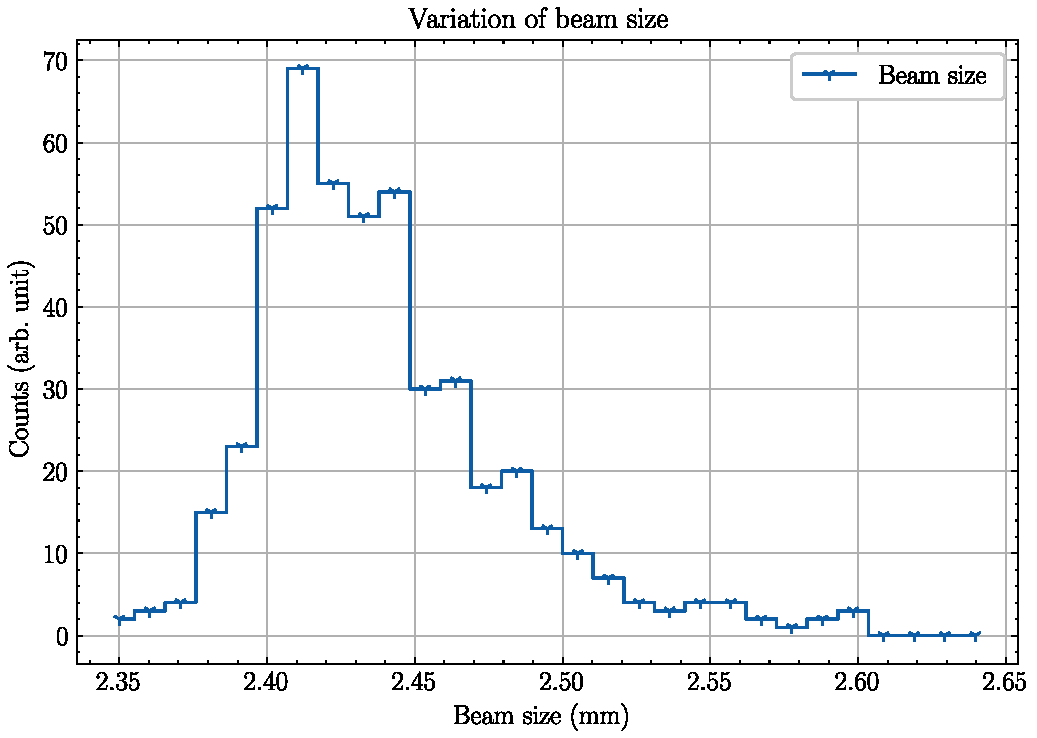
\includegraphics[width=1\textwidth]{04_Test/fig/fig000_hist_variation_b}
    \end{column}
  \end{columns}
\end{frame}

\begin{frame}
  \frametitle{Limitations}
  \begin{columns}[T]
    \begin{column}{0.45\textwidth}
      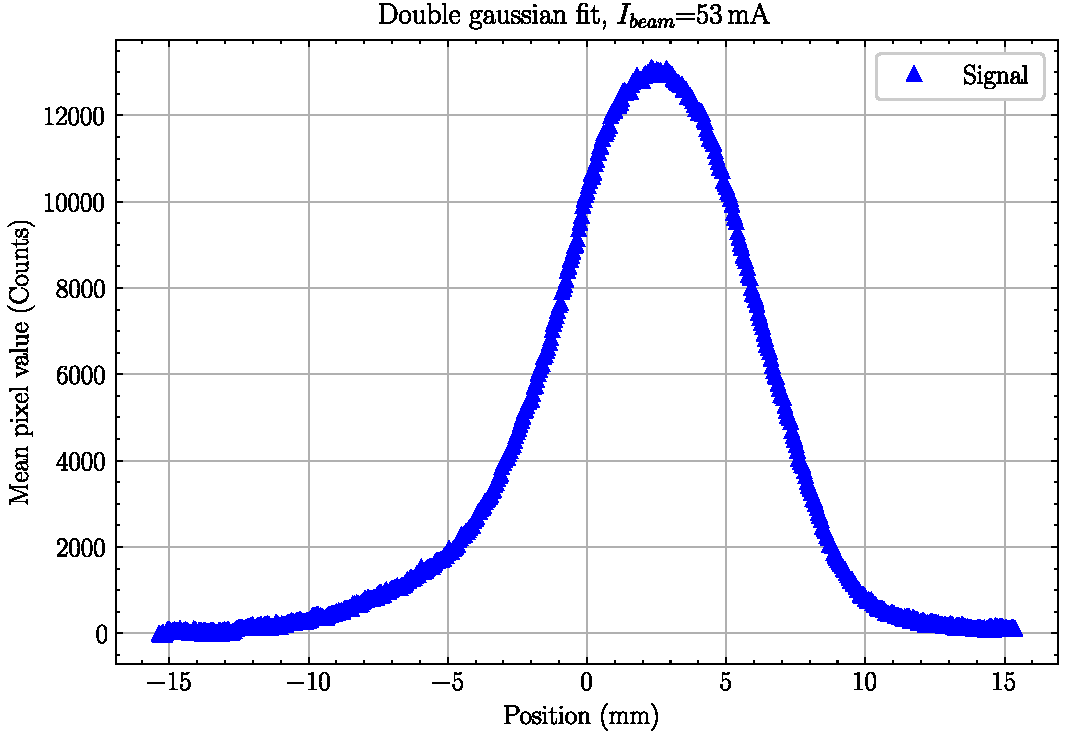
\includegraphics[width=1\textwidth]{04_Test/fig/fig000_ex_beam_profile_a}
    \end{column}
    \begin{column}{0.45\textwidth}
      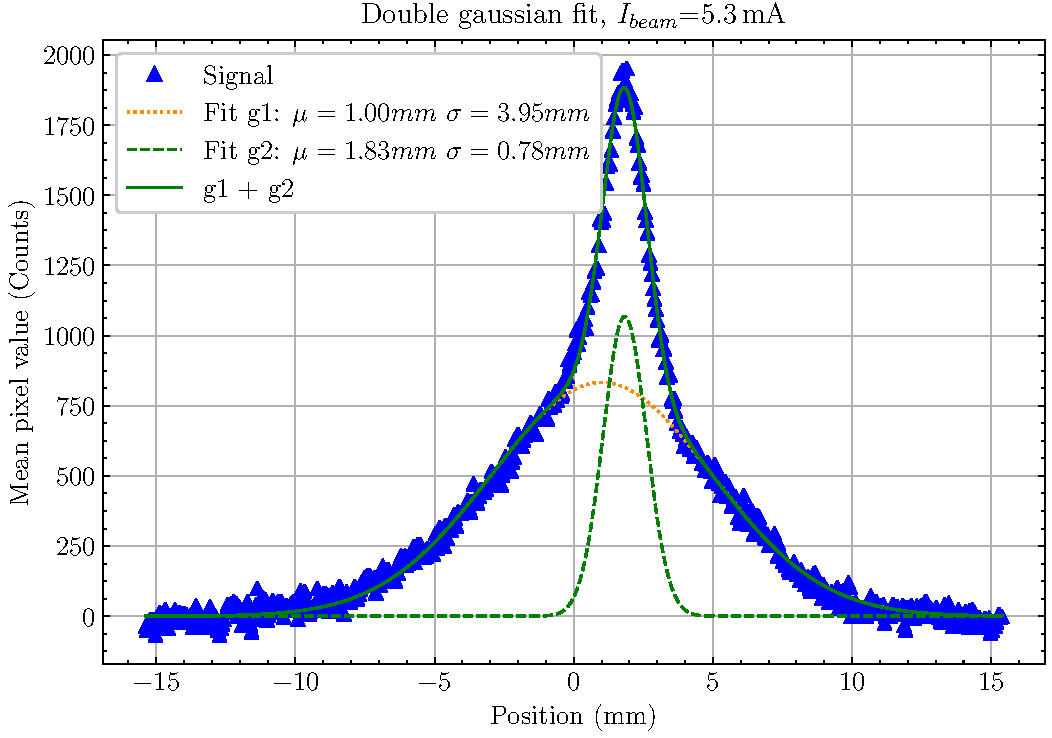
\includegraphics[width=1\textwidth]{04_Test/fig/fig000_ex_beam_profile_b2}
    \end{column}
  \end{columns}
  \begin{alertblock}{Precise measurements were not possible}
    \begin{itemize}
      \item Important position variation $\implies$ influence on size too?
      \item Beam shape depends on current $\implies$ How to quantify size?
    \end{itemize}
  \end{alertblock}
\end{frame}

\begin{frame}
  \frametitle{Comparison with IHPI diagnostic}
  \begin{alertblock}{No profile monitor available at IPHI}
    Impossible to compare the profile measured by IPM $\implies$ compare other quantities
  \end{alertblock}
  \begin{columns}[T]
    \begin{column}{0.45\textwidth}
      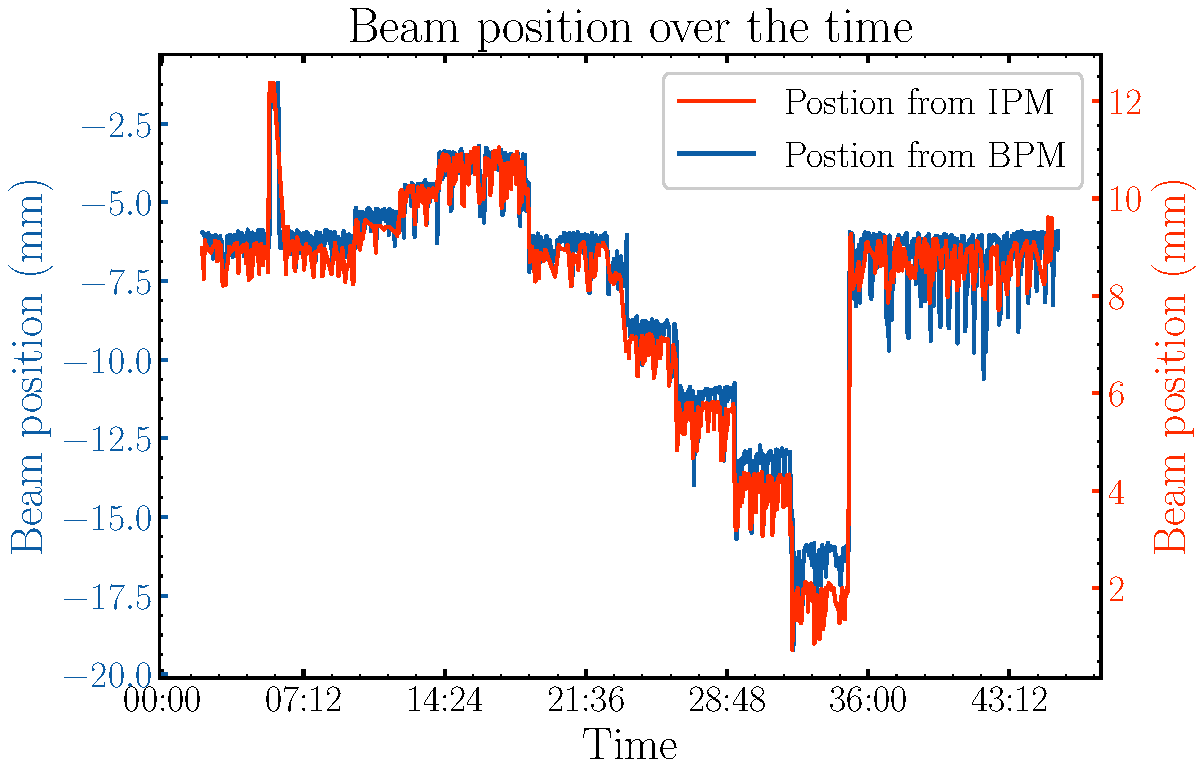
\includegraphics[width=1.14\textwidth]{04_Test/fig/fig000_beam_car_a}
    \end{column}
    \begin{column}{0.45\textwidth}
      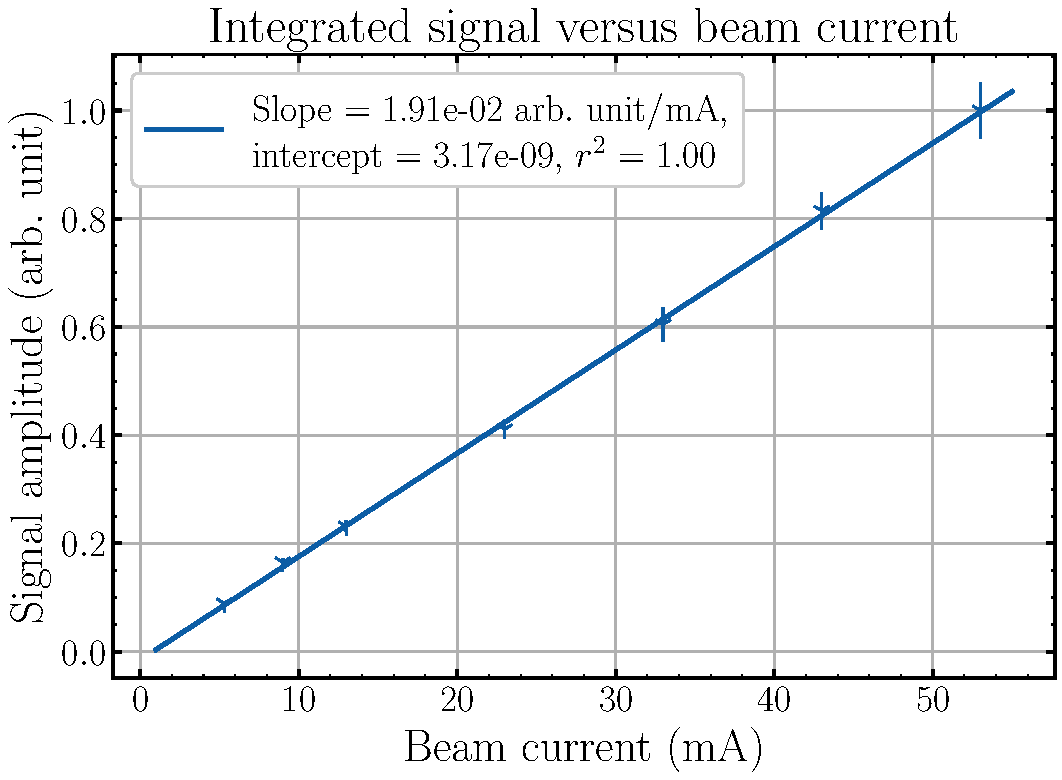
\includegraphics[width=1\textwidth]{04_Test/fig/fig000_current_sweep_a}
    \end{column}
  \end{columns}
  \begin{columns}[T]
    \begin{column}{0.45\textwidth}
      \begin{block}{Position with BPM}
        \begin{itemize}
          \item Step variation: steerers
          \item Correlation
        \end{itemize}
      \end{block}
    \end{column}
    \begin{column}{0.45\textwidth}
      \begin{block}{Current with DCCT}
        \begin{itemize}
          \item Linear response
          \item Important range
        \end{itemize}
      \end{block}
    \end{column}
  \end{columns}
\end{frame}

% \begin{frame}
%   \frametitle{Field uniformity}
%   \begin{alertblock}{}
%   \end{alertblock}
% \end{frame}

\begin{frame}
  \frametitle{MCP system characterization}
  \begin{columns}[T]
    \begin{column}{0.45\textwidth}
          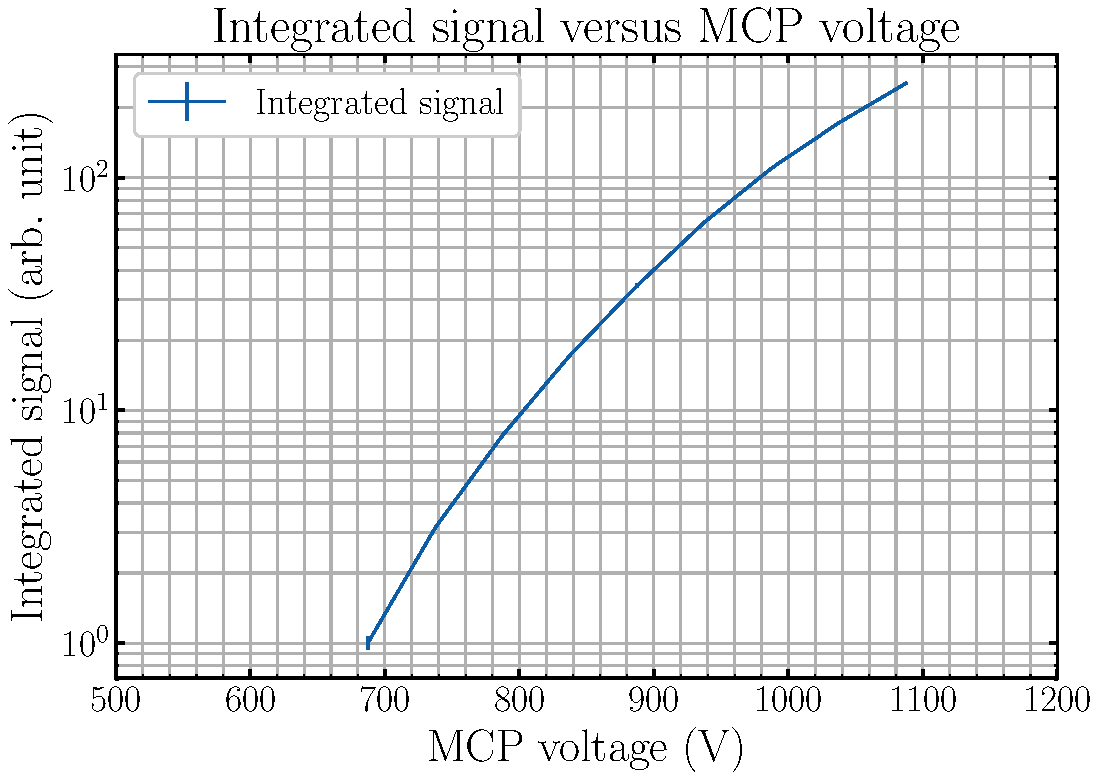
\includegraphics[width=1\textwidth]{04_Test/fig/fig000_MCP_gain_a}
          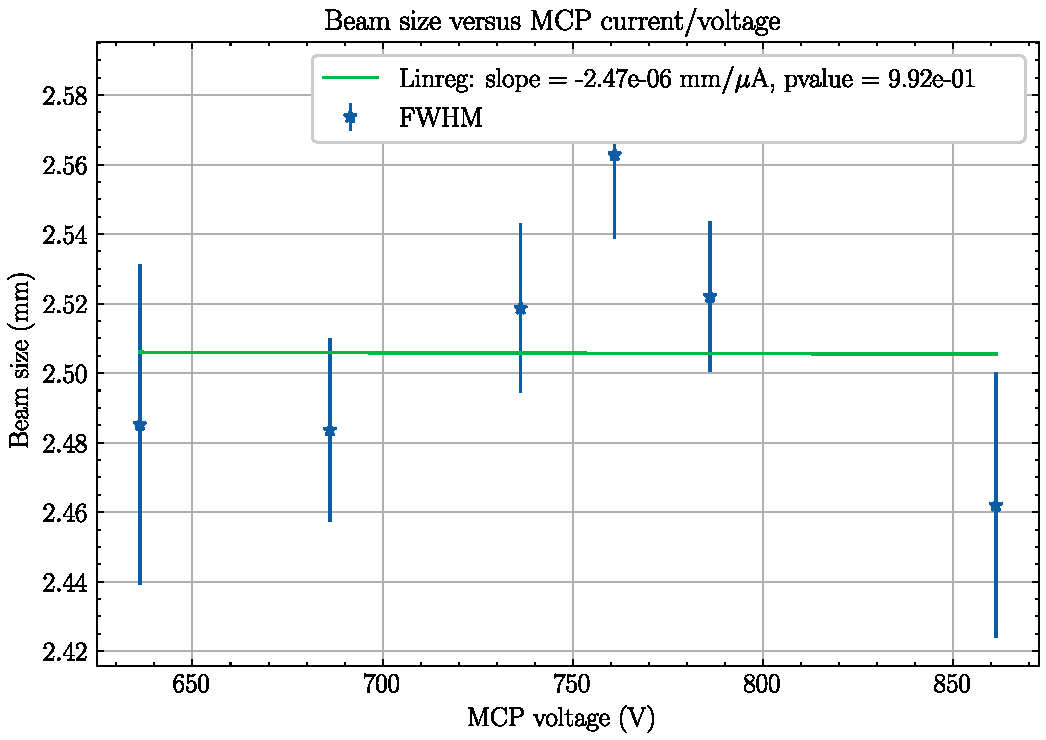
\includegraphics[width=1\textwidth]{04_Test/fig/fig000_MCP_gain_b}
    \end{column}
    \begin{column}{0.45\textwidth}
      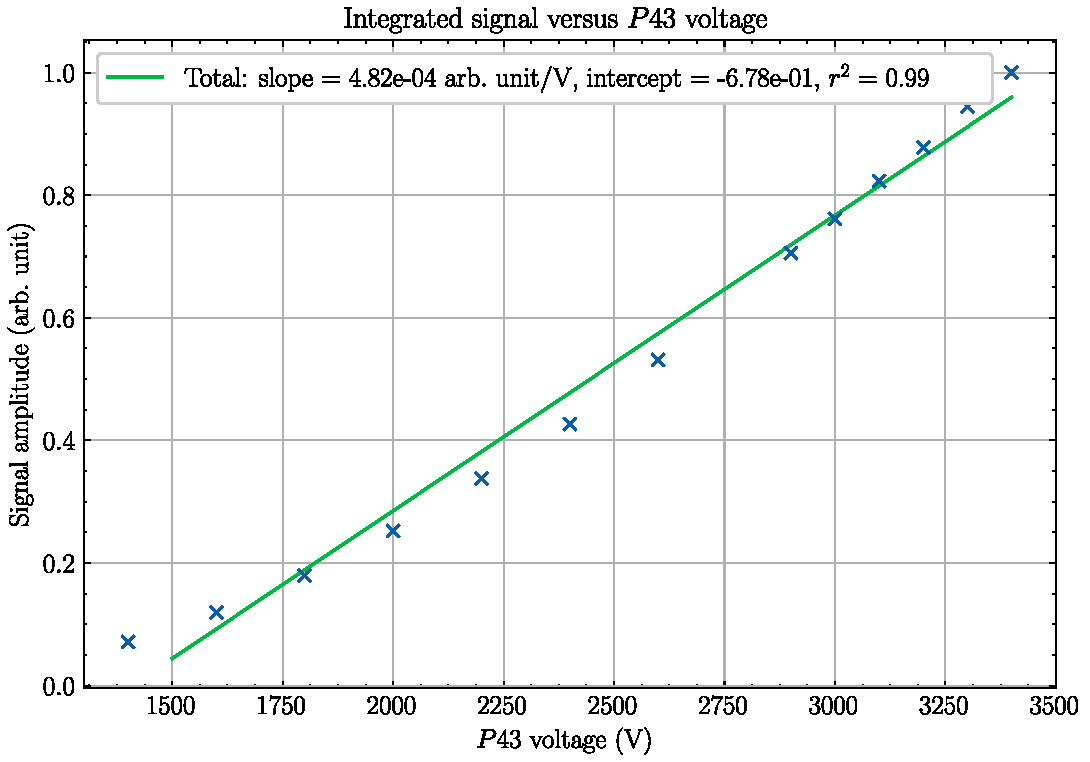
\includegraphics[width=1\textwidth]{04_Test/fig/fig000_P43_gain}
      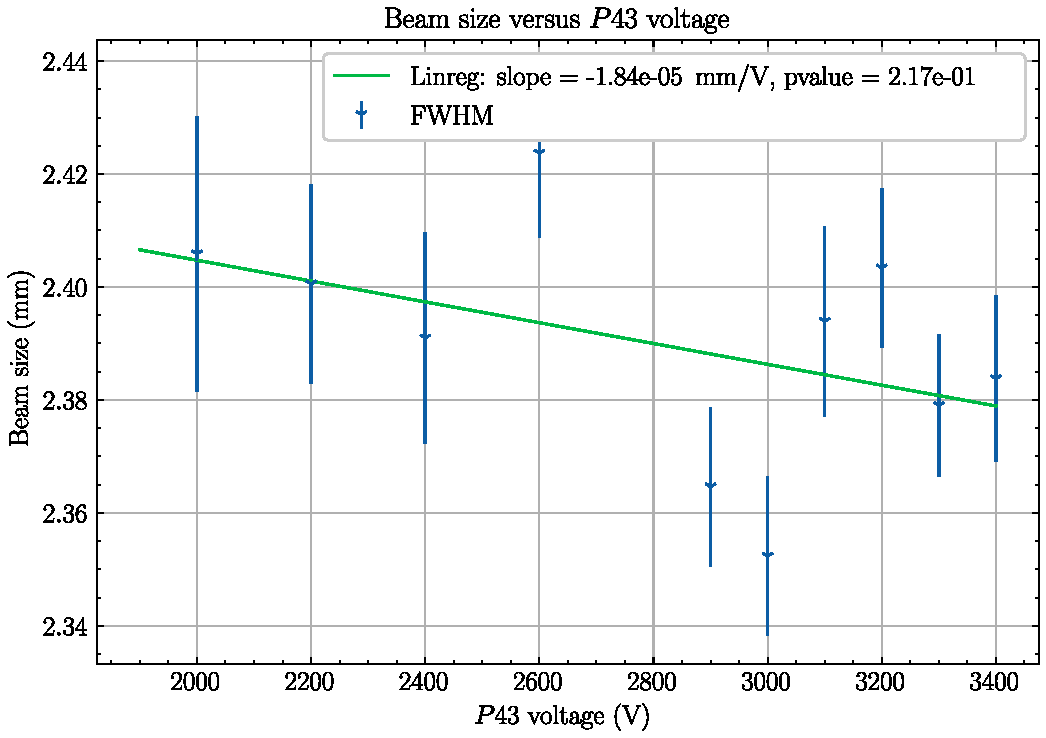
\includegraphics[width=1\textwidth]{04_Test/fig/fig000_P43_size}
    \end{column}
  \end{columns}
\end{frame}

\begin{frame}
  \frametitle{Phosphorus screen}
  \begin{columns}[T]
    \begin{column}{0.45\textwidth}
      \begin{block}{}
      \end{block}
    \end{column}
    \begin{column}{0.45\textwidth}
      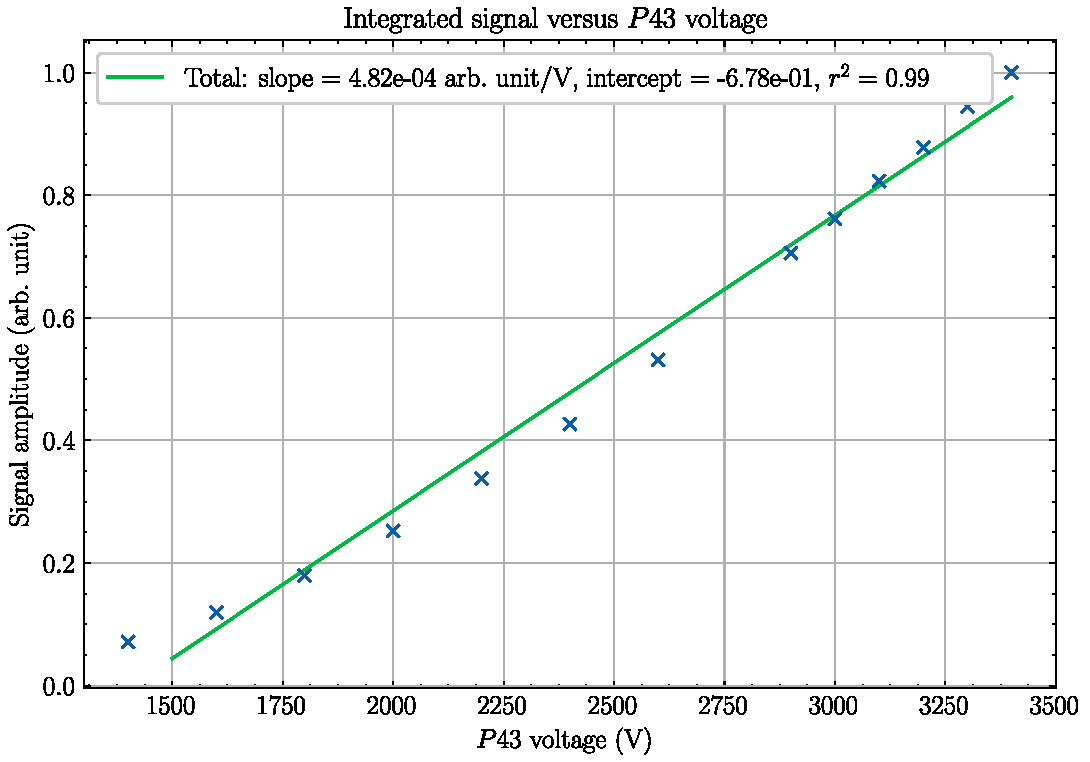
\includegraphics[width=1\textwidth]{04_Test/fig/fig000_P43_gain}
      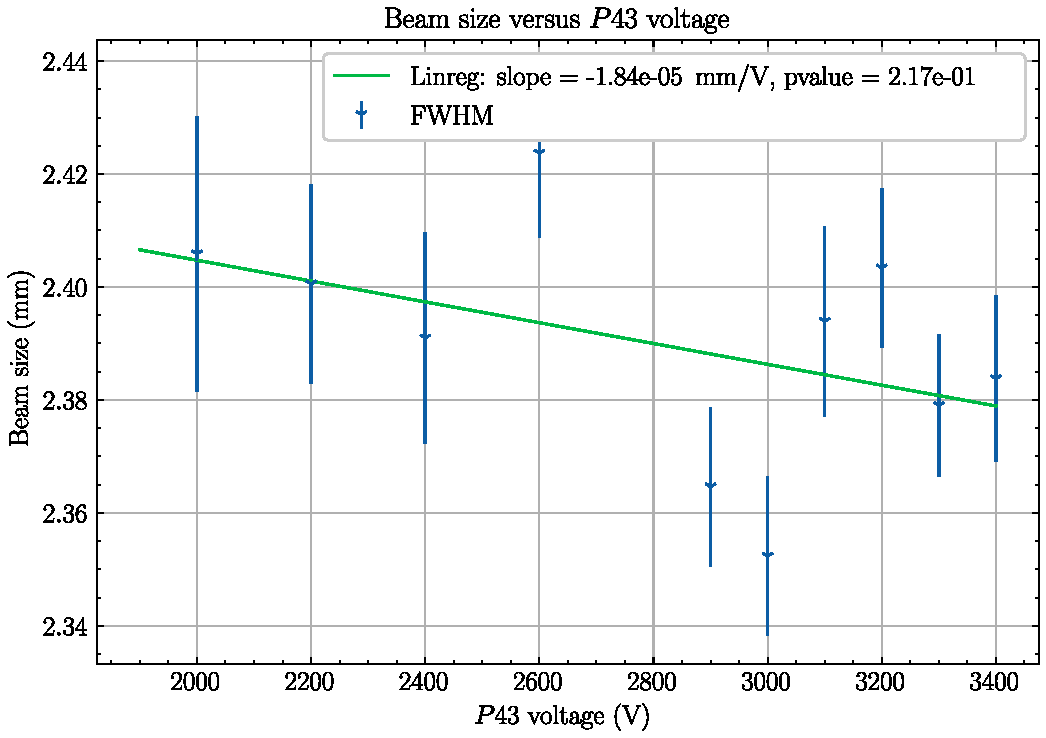
\includegraphics[width=1\textwidth]{04_Test/fig/fig000_P43_size}
    \end{column}
  \end{columns}
\end{frame}

\begin{frame}
  \frametitle{Limits of detection}
  \begin{columns}[T]
    \begin{column}{0.35\textwidth}
      \begin{block}{Signal at IPHI is higher:}
        \begin{itemize}
          \item Lower beam energy $\implies$ higher cross section
          \item Lower vacuum level
        \end{itemize}
        But can be compensated by:
        \begin{itemize}
          \item Reducing the current
          \item Reducing the pulse duration
        \end{itemize}
      \end{block}
    \end{column}
    \begin{column}{0.55\textwidth}
      \centering
      \includegraphics[width=1\textwidth]{04_Test/fig/fig000_bethe}
    \end{column}
  \end{columns}

  \begin{columns}[T]
    \begin{column}{0.45\textwidth}
      \begin{block}{Limits with strips}
      \end{block}
    \end{column}
    \begin{column}{0.45\textwidth}

    \end{column}
  \end{columns}
  \begin{alertblock}{Conclusion}
    Bare strips may not be able to detect at ESS.
  \end{alertblock}
\end{frame}

\begin{frame}
  \frametitle{Limits of detection}
  \begin{columns}[T]
    \begin{column}{0.45\textwidth}
      \begin{block}{Limits with MCP}
        With MCP IPM we reached the limits of IPHI:
        \begin{itemize}
          \item $0.5\,\mathrm{mA}$ and $100\,\mathrm{\mu s}$
          \item Equivalent to worst ESS case at $2\,\mathrm{GeV}$
        \end{itemize}
      \end{block}
    \end{column}
    \begin{column}{0.45\textwidth}
      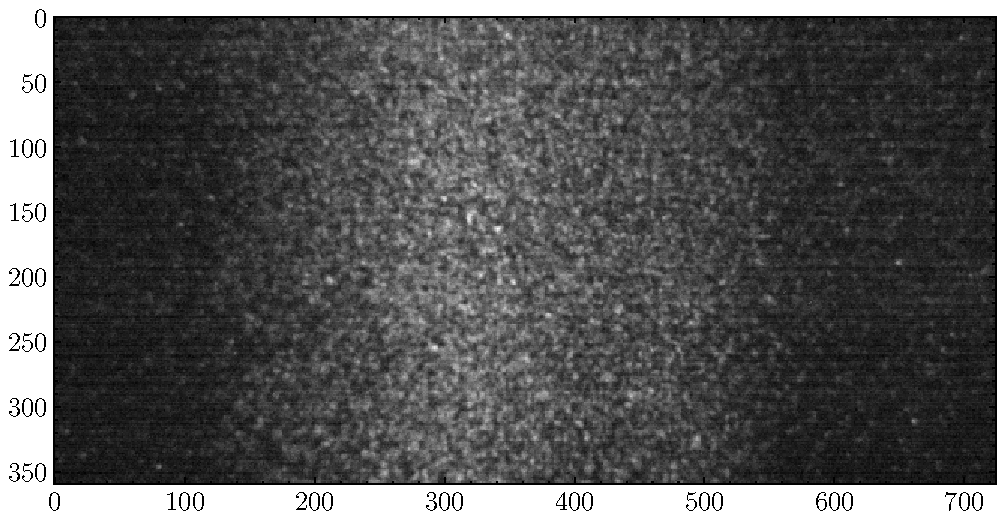
\includegraphics[width=1\textwidth]{04_Test/fig/fig000_limits_IPHI_a}
      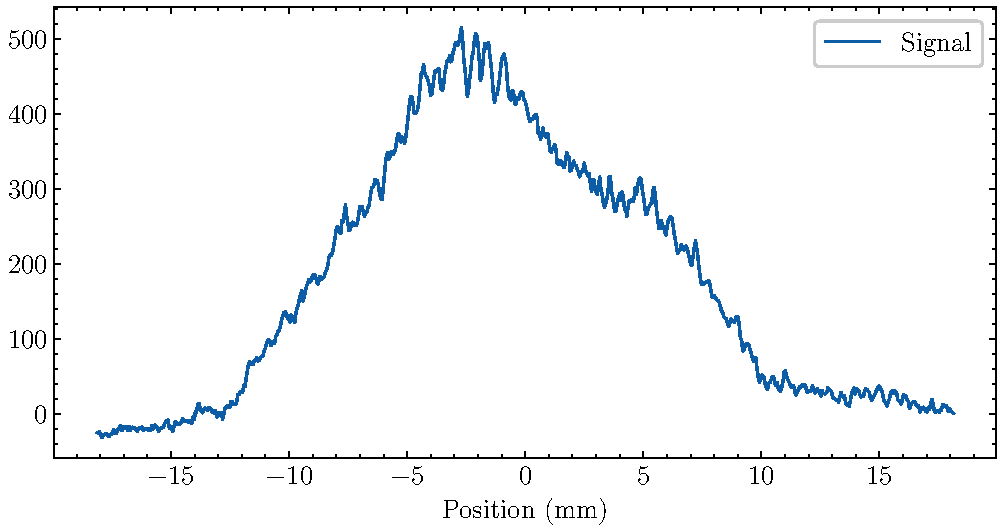
\includegraphics[width=1\textwidth]{04_Test/fig/fig000_limits_IPHI_b}
    \end{column}
  \end{columns}
  \begin{alertblock}{Conclusion}
    Even a single stage MCP seems to be sufficient to detect profile.
  \end{alertblock}
\end{frame}